%!TEX TS-program = xelatex
%!TEX encoding = UTF-8 Unicode
\documentclass[a4paper,twocolumn]{article}
\usepackage[scale=.85]{geometry}
\usepackage{graphicx}
\usepackage[no-math]{fontspec}
\usepackage[colorlinks,linktoc=page,unicode]{hyperref}
\usepackage{pstricks-add}
\usepackage[CJKnumber]{xeCJK}

\setCJKmainfont[AutoFakeBold,ItalicFont=AR PL UKai TW]{AR PL UMing TW}
\setCJKsansfont[AutoFakeBold,ItalicFont=AR PL UKai TW]{WenQuanYi Zen Hei}
\setlength{\parindent}{2em}

\renewcommand{\figurename}{圖}

\begin{document}
\title{小鼠的骨骼肌型態觀察}
\author{B101100025 何震邦}
\date{2014 年 5 月 27 日}
\maketitle

\section{目的}
藉由觀察其他哺乳動物的組織型態,以最經濟的方式培養未來行醫判讀人體組織切片的能
力。

\section{簡介}
本實驗取小鼠的組織做成石蠟切片,並取相近的兩片進行 H\&E 與 Masson trichrome 染
色。觀察的片子是其他同學製作的,所以我們必須在顯微鏡下判讀該片是什麼組織。

\section{材料與方法}
\subsection{固定}
固定指的是避免組織降解,並維持細胞與胞器的結構。因為我們要做石蠟切片,所以採取
化學固定,也就是使用 10\% 中性福馬林緩衝溶液 (neutral buffered formalin),即在
磷酸鹽緩衝生理食鹽水 (phosphate buffered saline, PBS) 中溶有 4\% 甲醛。

\subsection{處理}
處理組織的目的是以固態物質取代組織中的水,使得組織可以被切薄。生物組織需要在夠
硬的基質中才能切成薄約 5 $\mu$m 的切片,以適於在光學顯微鏡下觀察。石蠟是最常用
的基質。因為石蠟不溶於水,也就是組織的主要成份,我們首先要把組織脫水。樣本先透
過幾個逐漸加濃的酒精浴脫水,接著再利用疏水溶劑,如二甲苯 (xylene),移除酒精,最
後再由熔融的石蠟取代二甲苯。

\subsection{包埋}
當組織的水份已充分被基質取代時,我們就用相同的物質包裏樣本。此時我們把樣本置入
熔融的石蠟中,再放涼使其固化。

因為以福馬林固定、石蠟包埋 (formalin-fixed, paraffin-embedded, FFPE) 的組織可在
室溫下無限期儲存,而且即使在固定的數十年後仍可取出核酸(包括 DNA 與 RNA),所以
FFPE 組織是重要的醫學歷史研究資源。

\subsection{切片}
切片的法子相當有限。一般我們採用垂直切片。

對光學顯微而言,切片機切出約 5 $\mu$m 厚的切片,再掛載於載玻片。

\subsection{染色}
生物組織在光學或電子顯微鏡下的對比都不明顯。染色使得不同的組織產生對比,並重點
標示感興趣的特徵。

\subsubsection{H\&E 染色}
H\&E 染色是最常用於組織、病理的光學顯微染色。鹼性藍色的蘇木精
(hematoxylin) 趨向酸性的核酸;酸性的伊紅 (eosin) 則把細胞質染成粉紅。

\subsubsection{Masson's trichrome 染色}
顧名思義,這種染色方法會染出三種顏色,但其實用了四種染劑。
\begin{itemize}
    \item Weigert's hematoxylin 是三種溶液的混合物:氯化鐵 (III) 溶於稀鹽酸、蘇
        木精溶於 95\% 酒精,以及被硼砂鹼化的鐵氫化鉀。這個染劑會把核染黑。
    \item 溶液 A,也就是\textbf{細胞質染劑},有 fushin, peonceau 2R、冰醋酸及
        水。
    \item 溶液 B 含有磷鉬酸水溶液,長得像維他露 P。不飽和的有機化合物會把它還原
        為鉬藍。
    \item 溶液 C,也就是\textbf{纖維染劑}。通常使用藍色或綠色染劑。我們採用藍色
        的甲基藍。
\end{itemize}

\section{結果}
量尺以 $\mu$m 為單位,倍率為紙上圖形與實物的比。

\begin{figure}
    \begin{center}
        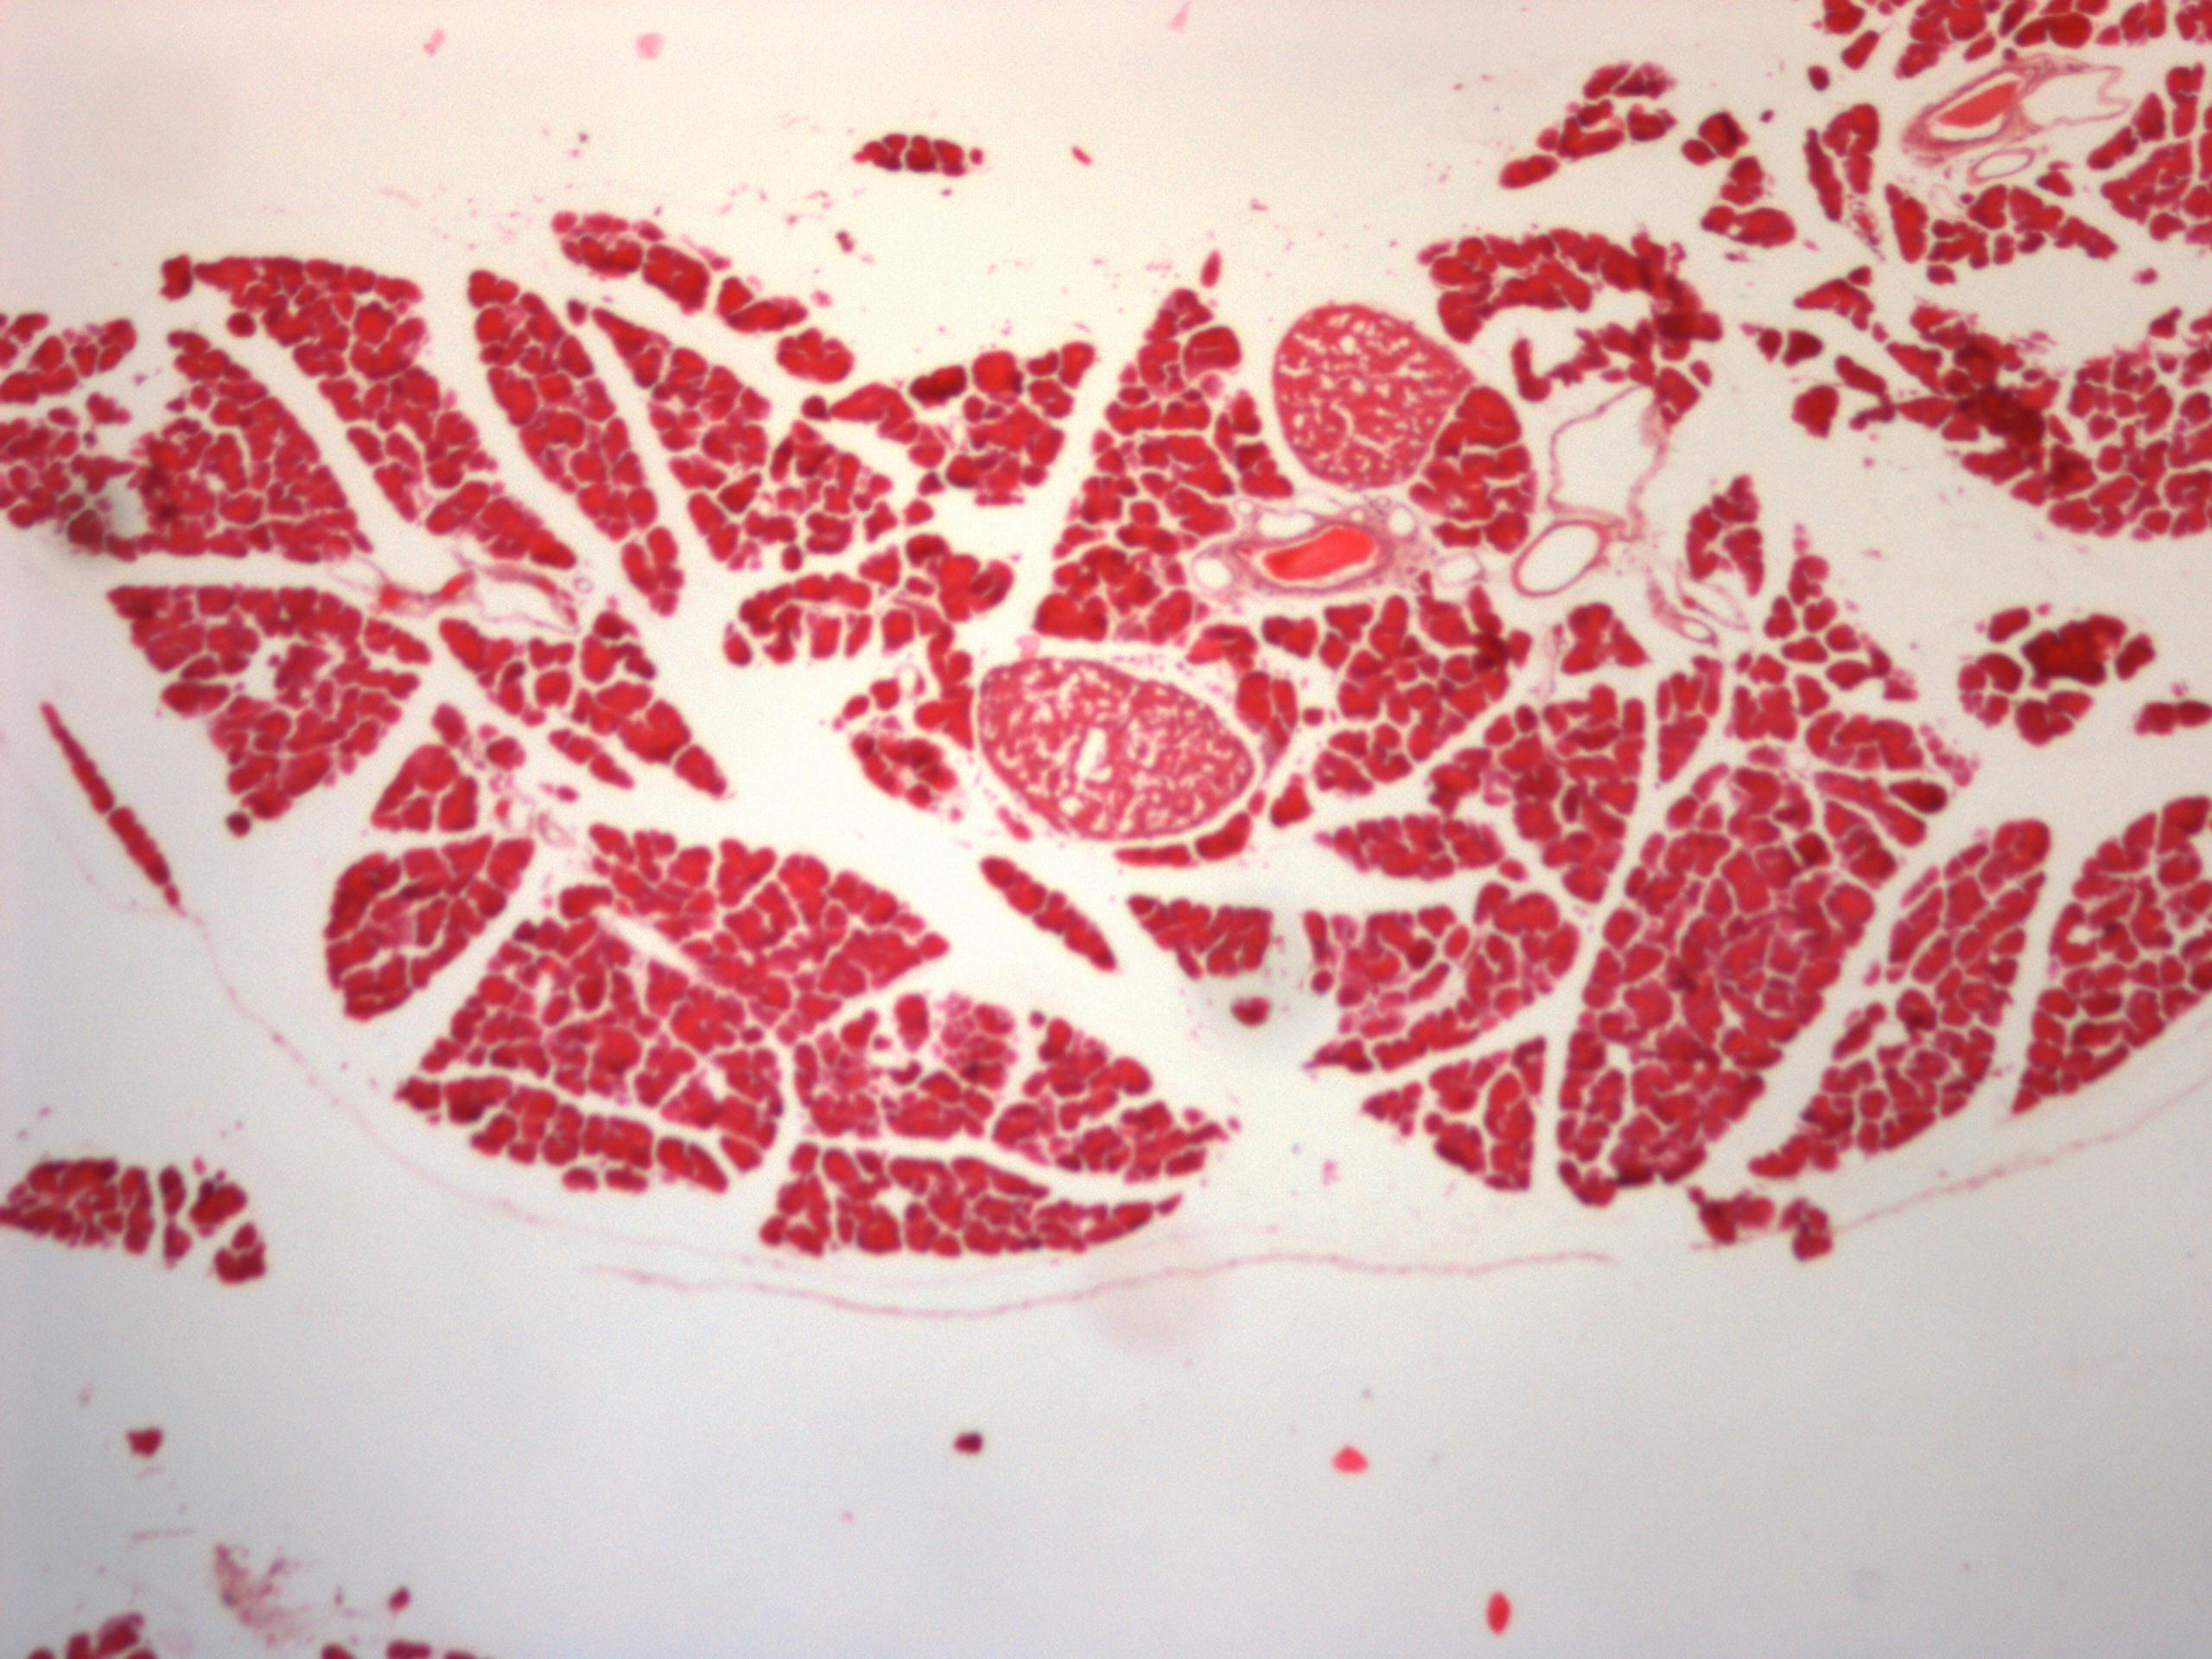
\includegraphics[width=86.2mm]{image/HE-4x.jpg}
    \end{center}
    \psset{unit=0.4mm}
    \begin{pspicture}(-2.5,-7.5)(97.5,-7.5)
        \psaxes[ticks=x,tickstyle=top,Dx= 5,ticksize=2.0mm,labels=none](0,0)(100,0)
        \psaxes[ticks=x,tickstyle=top,Dx=10,ticksize=3.5mm,labels=none](0,0)(100,0)
        \psaxes[ticks=none,Dx=20](0,0)(100,0)
    \end{pspicture}
    \caption{H\&E 40x}
\end{figure}

\begin{figure}
    \begin{center}
        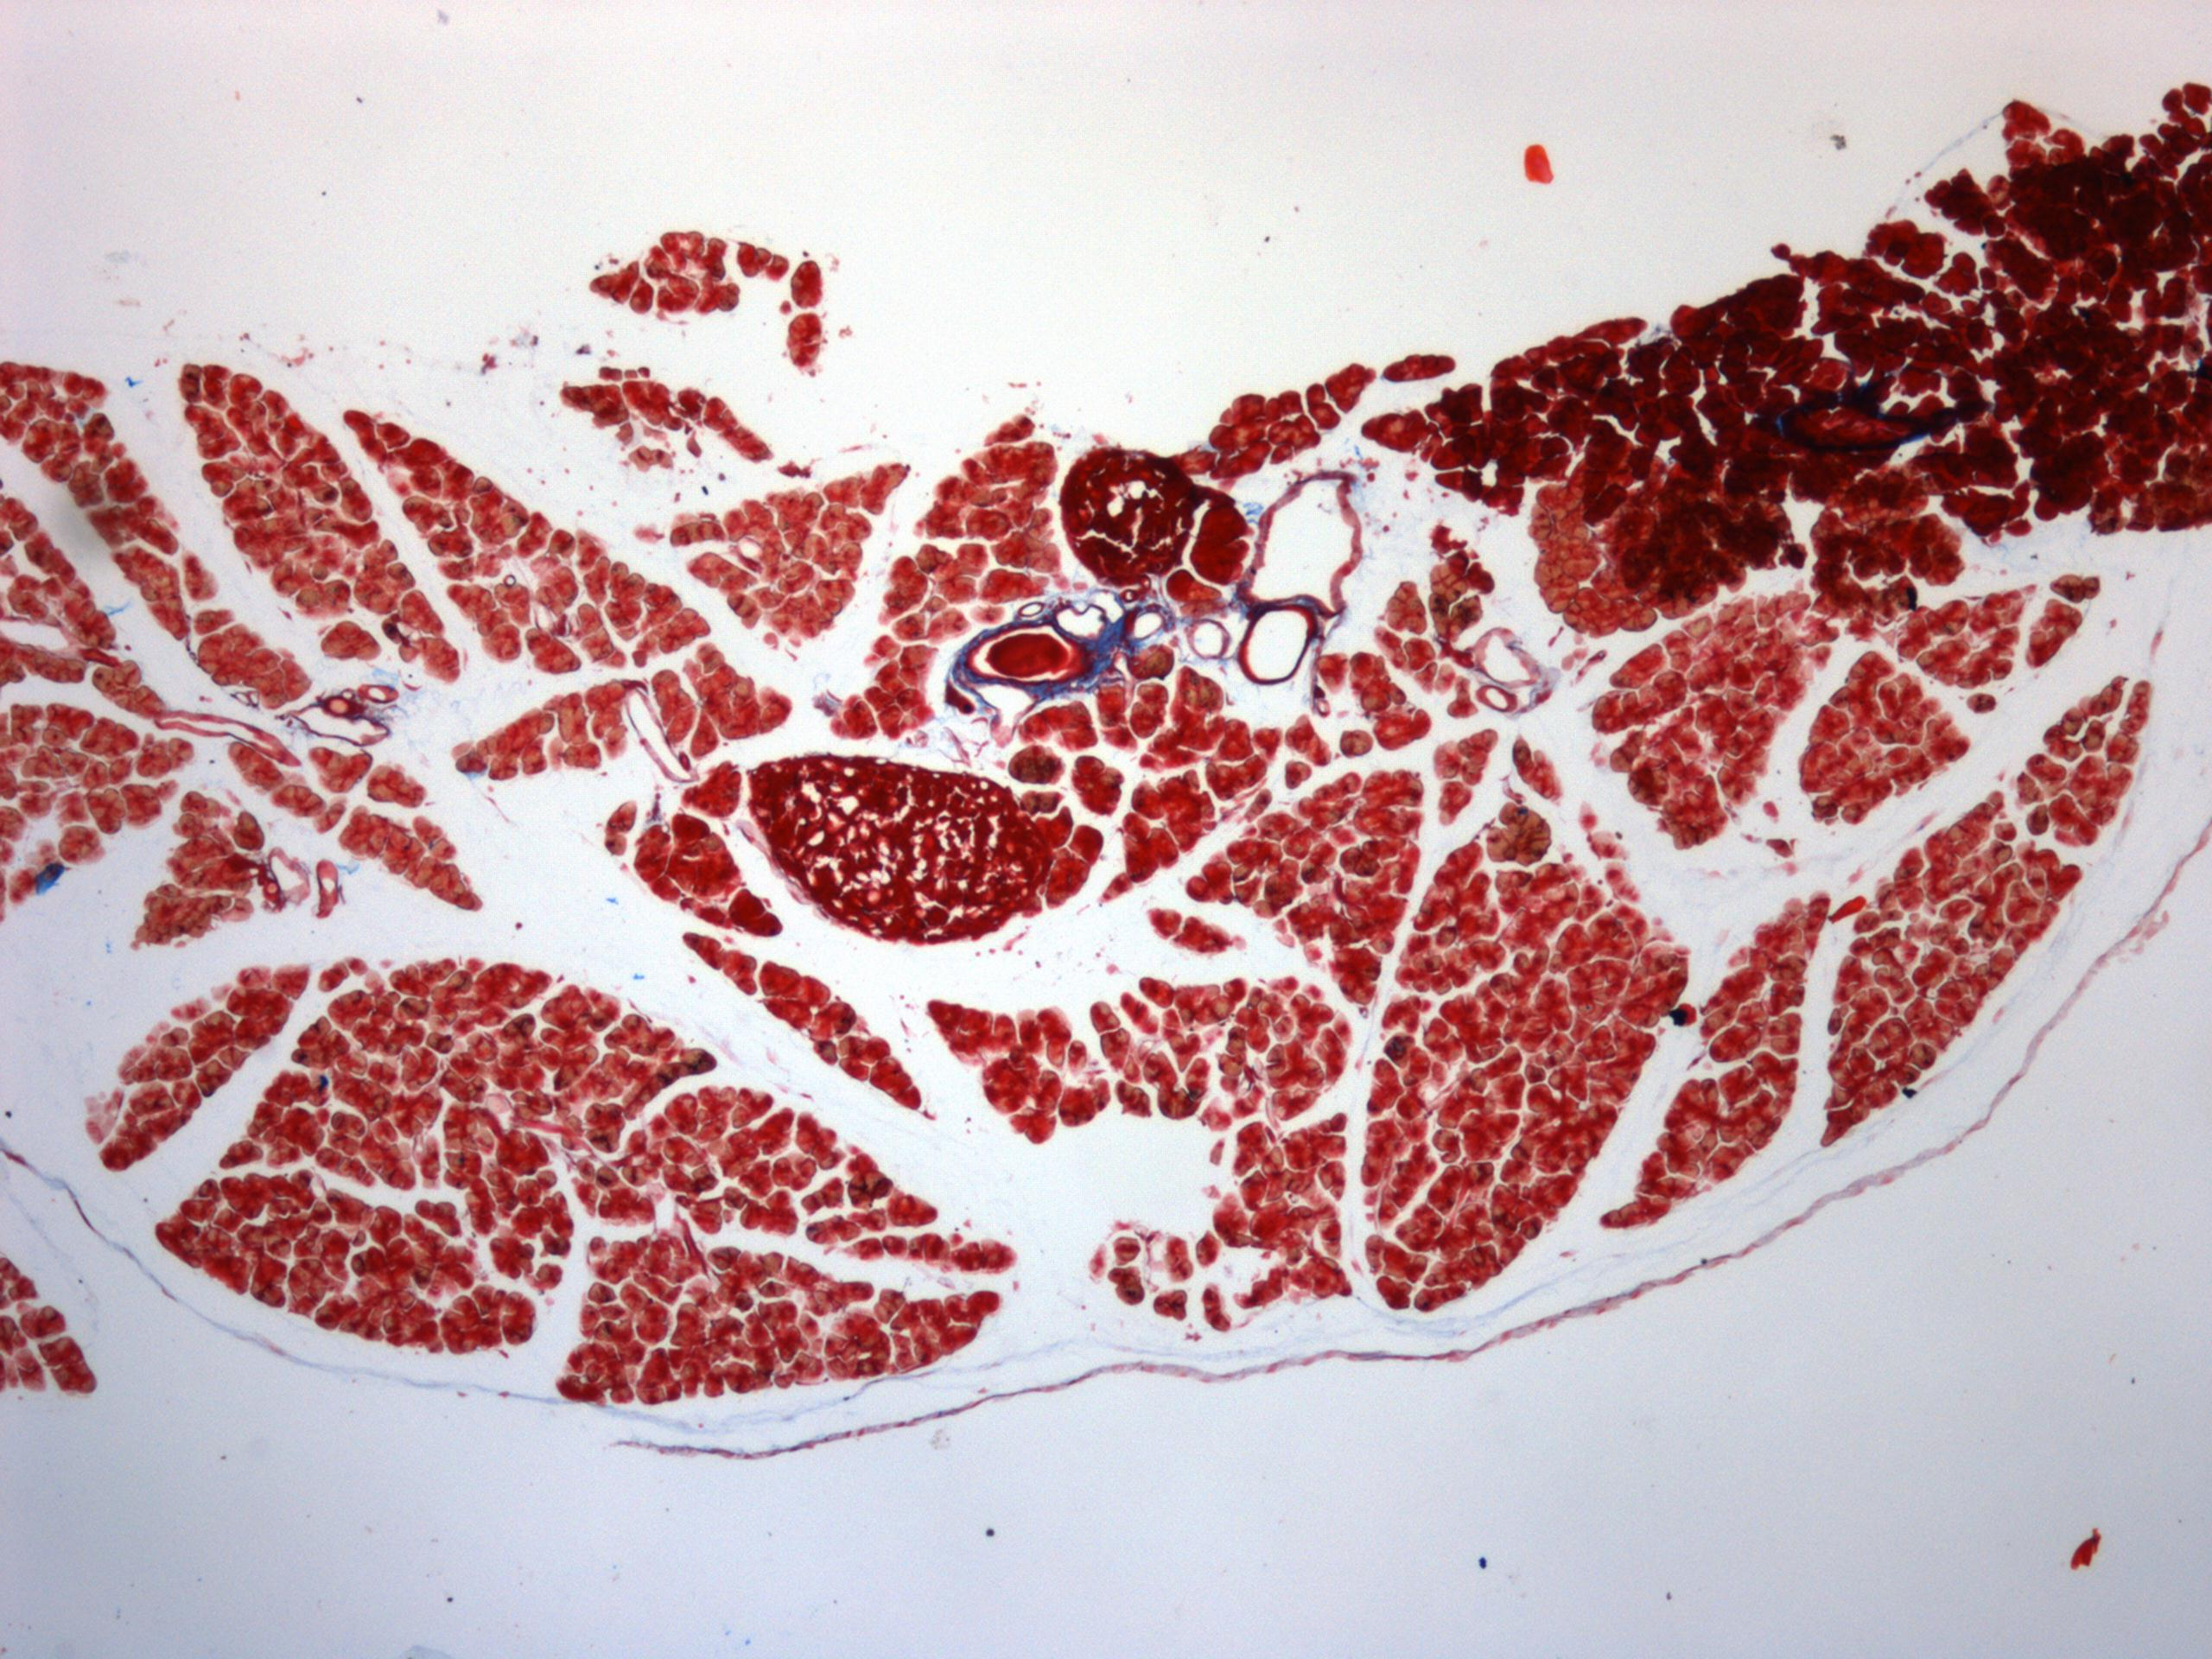
\includegraphics[width=86.2mm]{image/Tri-4x.jpg}
    \end{center}
    \psset{unit=0.4mm}
    \begin{pspicture}(-2.5,-7.5)(97.5,-7.5)
        \psaxes[ticks=x,tickstyle=top,Dx= 5,ticksize=2.0mm,labels=none](0,0)(100,0)
        \psaxes[ticks=x,tickstyle=top,Dx=10,ticksize=3.5mm,labels=none](0,0)(100,0)
        \psaxes[ticks=none,Dx=20](0,0)(100,0)
    \end{pspicture}
    \caption{Masson's trichrome 40x}
\end{figure}

\begin{figure}
    \begin{center}
        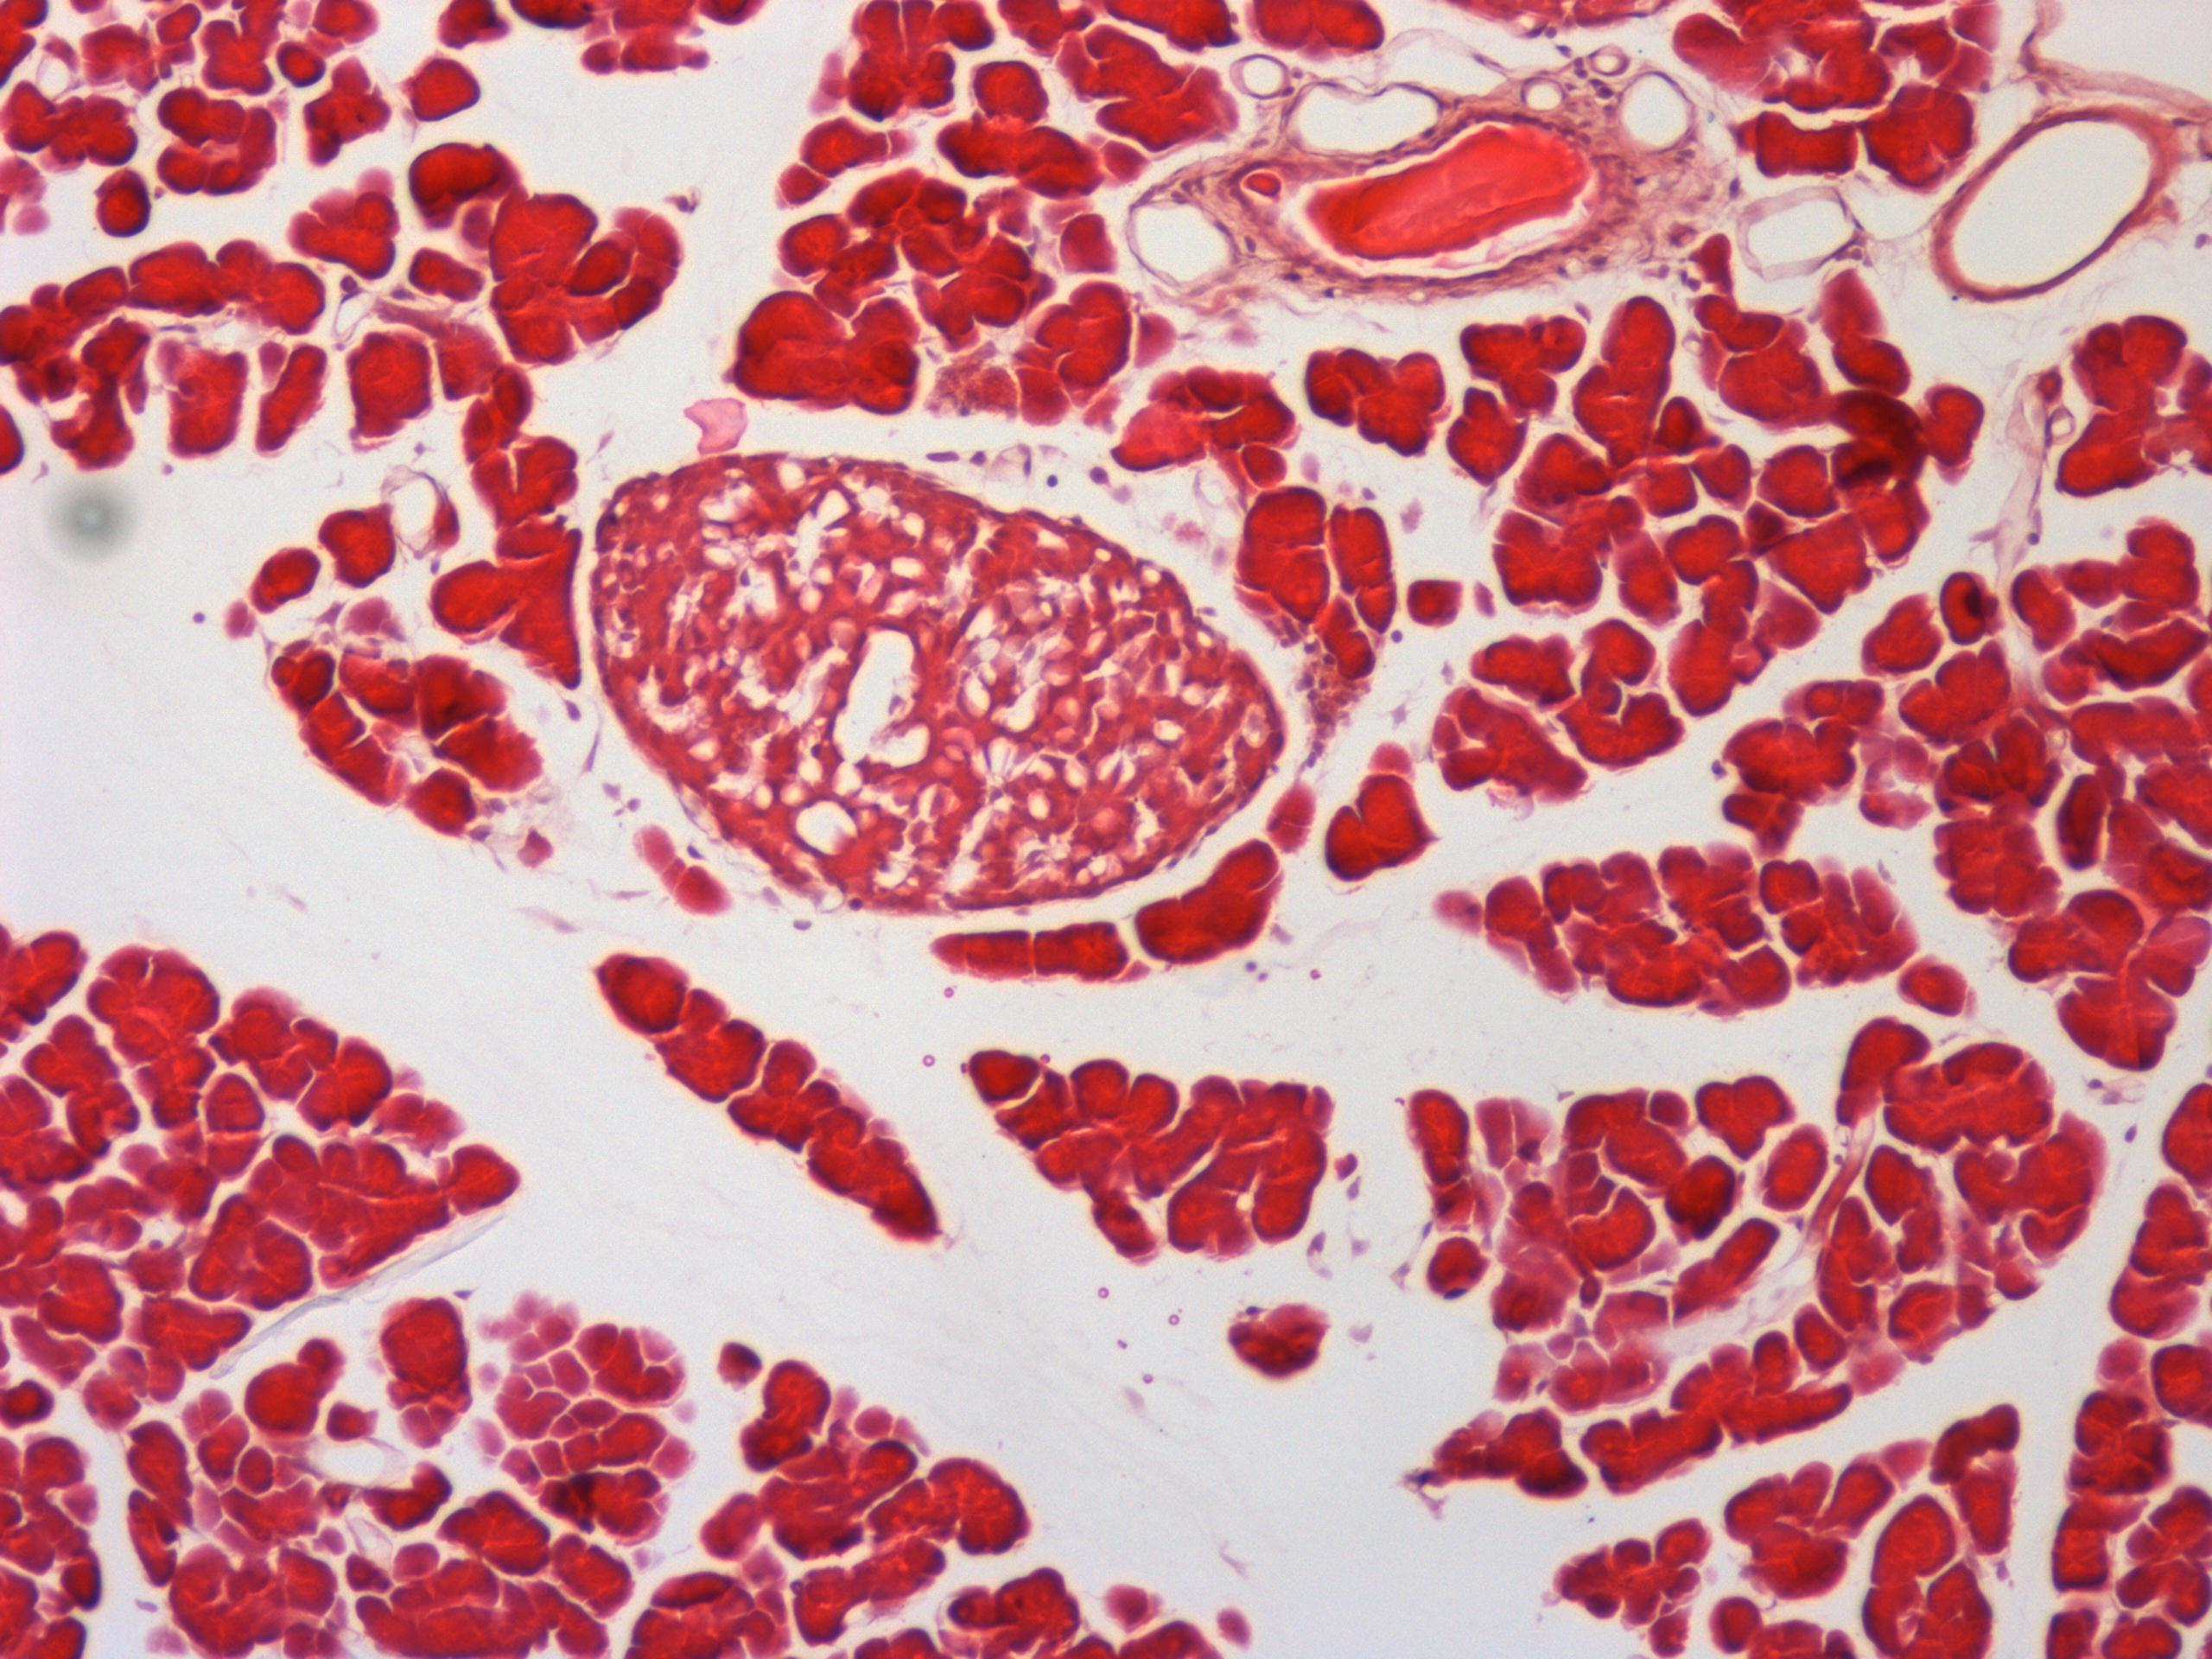
\includegraphics[width=86.2mm]{image/HE-10x.jpg}
    \end{center}
    \psset{unit=1mm}
    \begin{pspicture}(-1,-3)(39,-3)
        \psaxes[ticks=x,tickstyle=top,Dx= 1,ticksize=1.5mm,labels=none](0,0)(40,0)
        \psaxes[ticks=x,tickstyle=top,Dx= 5,ticksize=2.5mm,labels=none](0,0)(40,0)
        \psaxes[ticks=x,tickstyle=top,Dx=10,ticksize=3.5mm            ](0,0)(40,0)
    \end{pspicture}
    \caption{H\&E 100x}
\end{figure}

\begin{figure}
    \begin{center}
        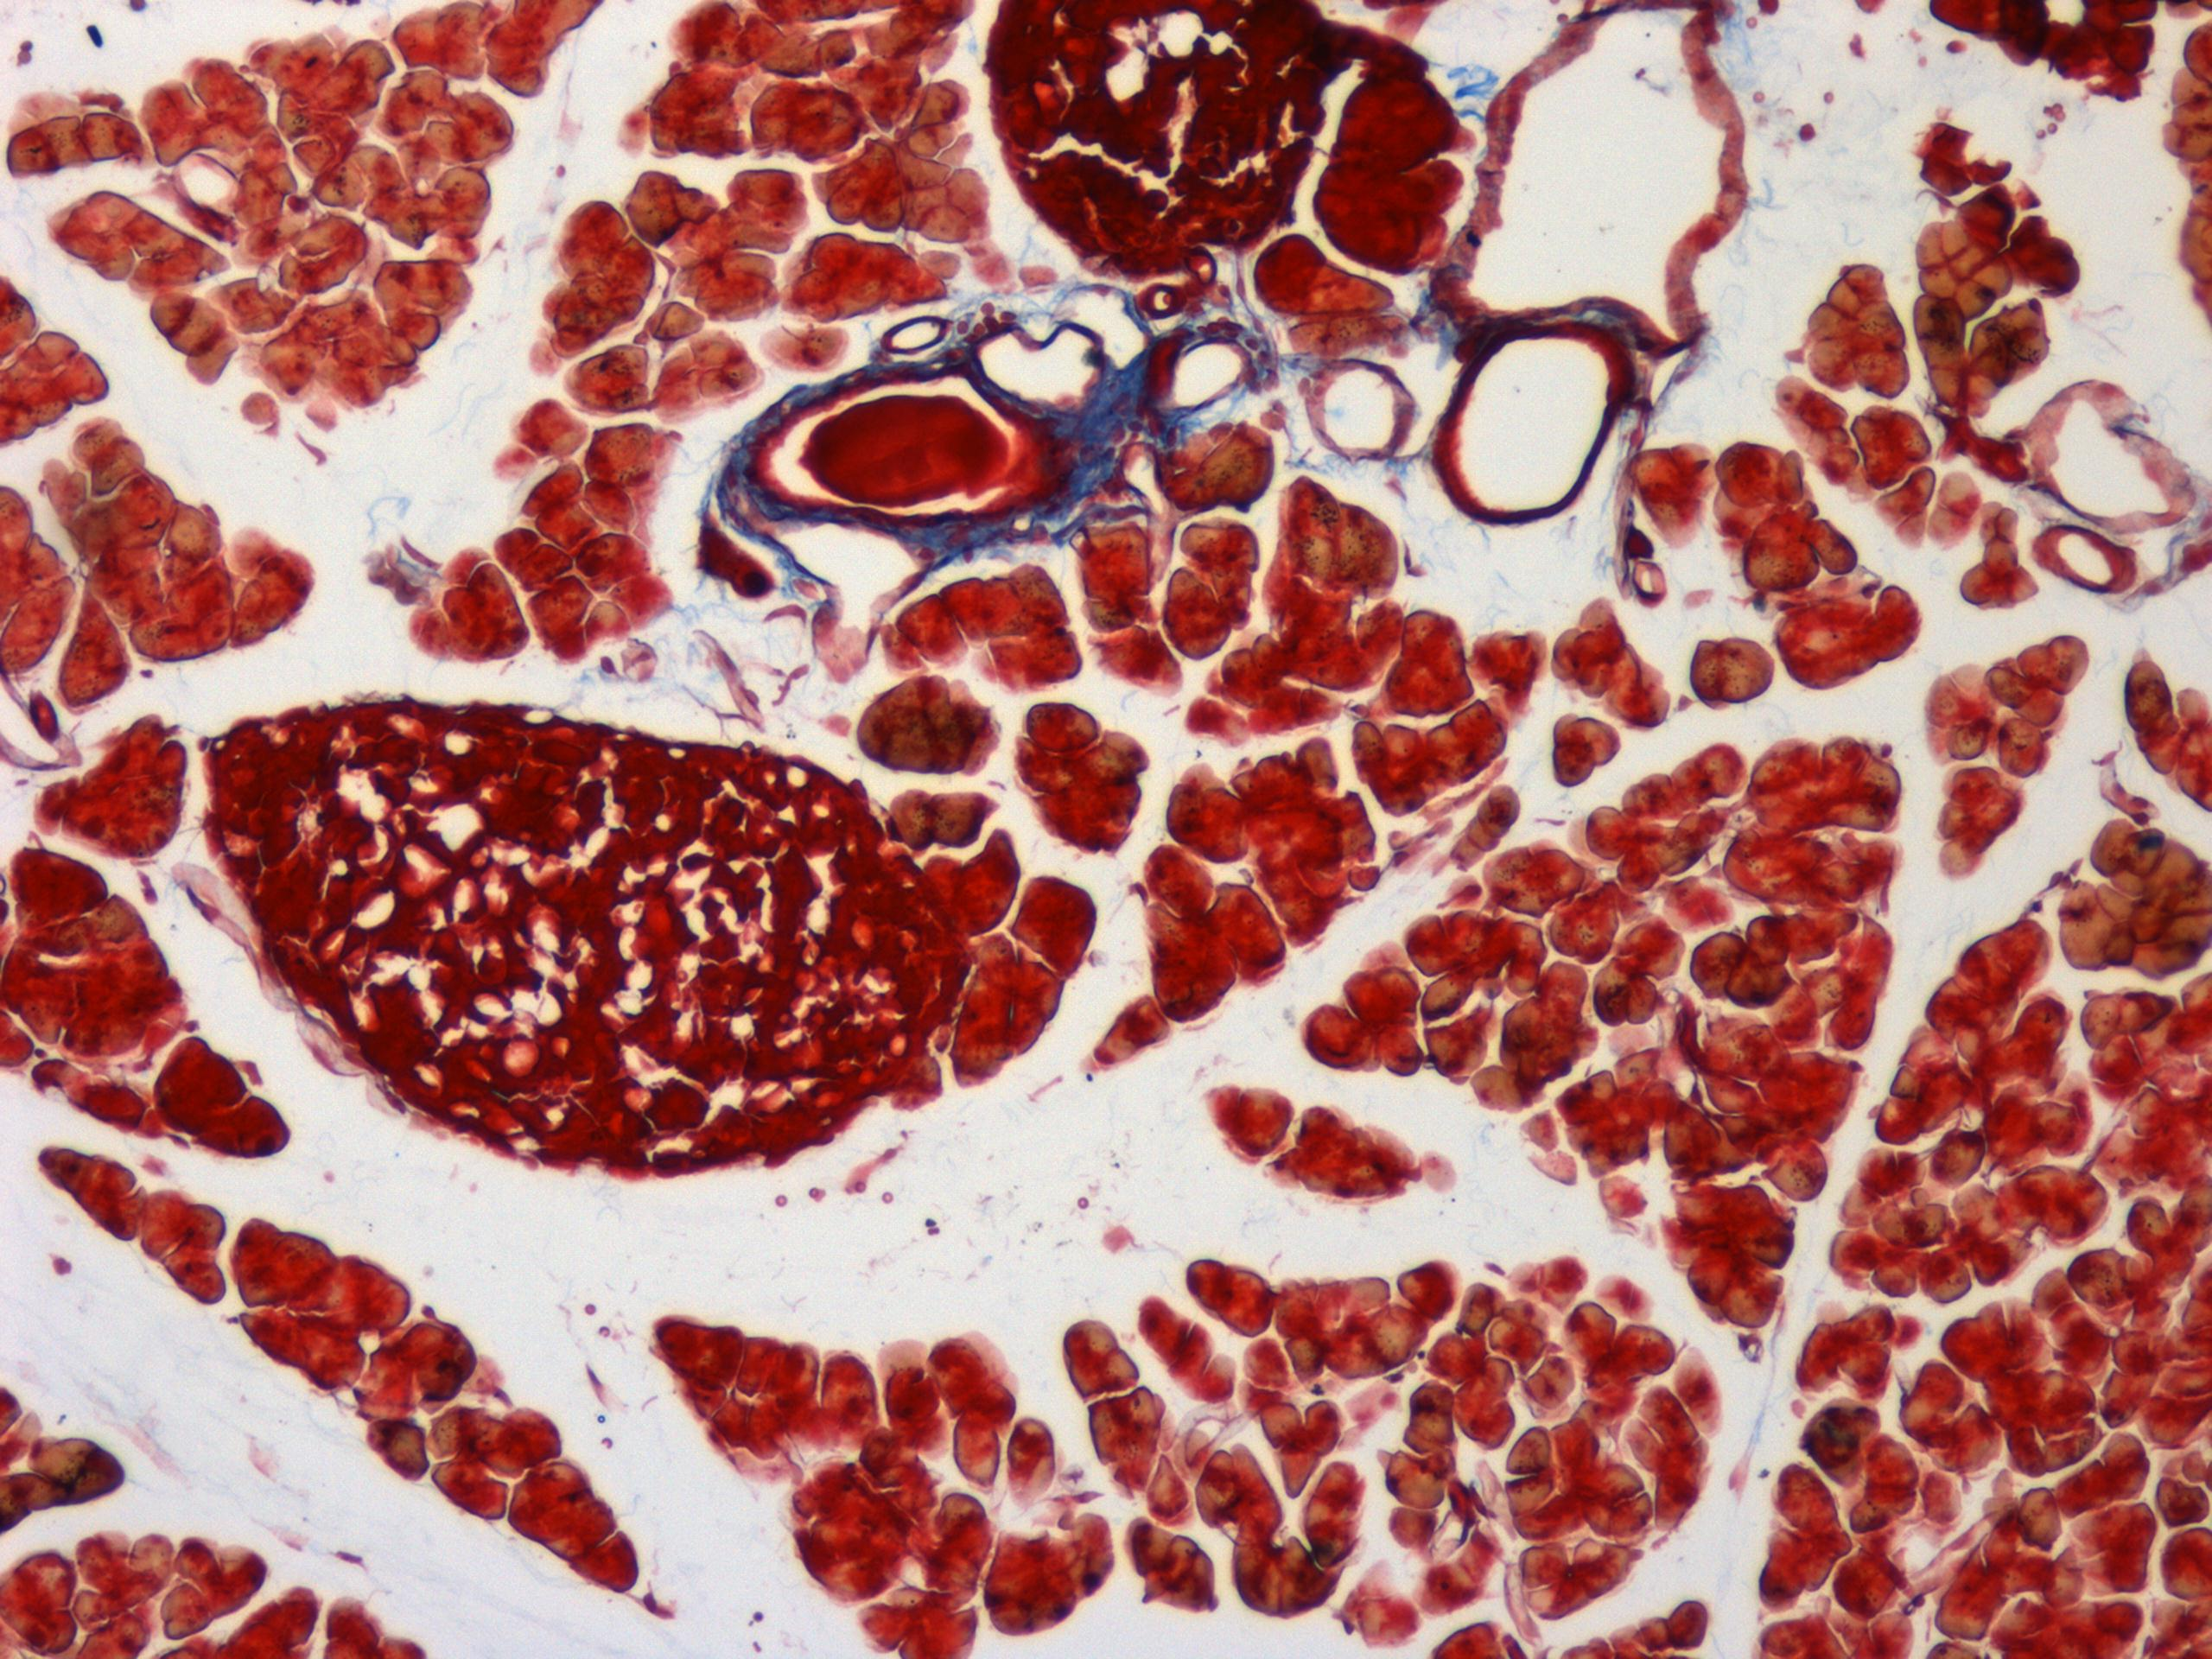
\includegraphics[width=86.2mm]{image/Tri-10x-1.jpg}
    \end{center}
    \psset{unit=1mm}
    \begin{pspicture}(-1,-3)(39,-3)
        \psaxes[ticks=x,tickstyle=top,Dx= 1,ticksize=1.5mm,labels=none](0,0)(40,0)
        \psaxes[ticks=x,tickstyle=top,Dx= 5,ticksize=2.5mm,labels=none](0,0)(40,0)
        \psaxes[ticks=x,tickstyle=top,Dx=10,ticksize=3.5mm            ](0,0)(40,0)
    \end{pspicture}
    \caption{Masson's trichrome 100x}
\end{figure}

\begin{figure}
    \begin{center}
        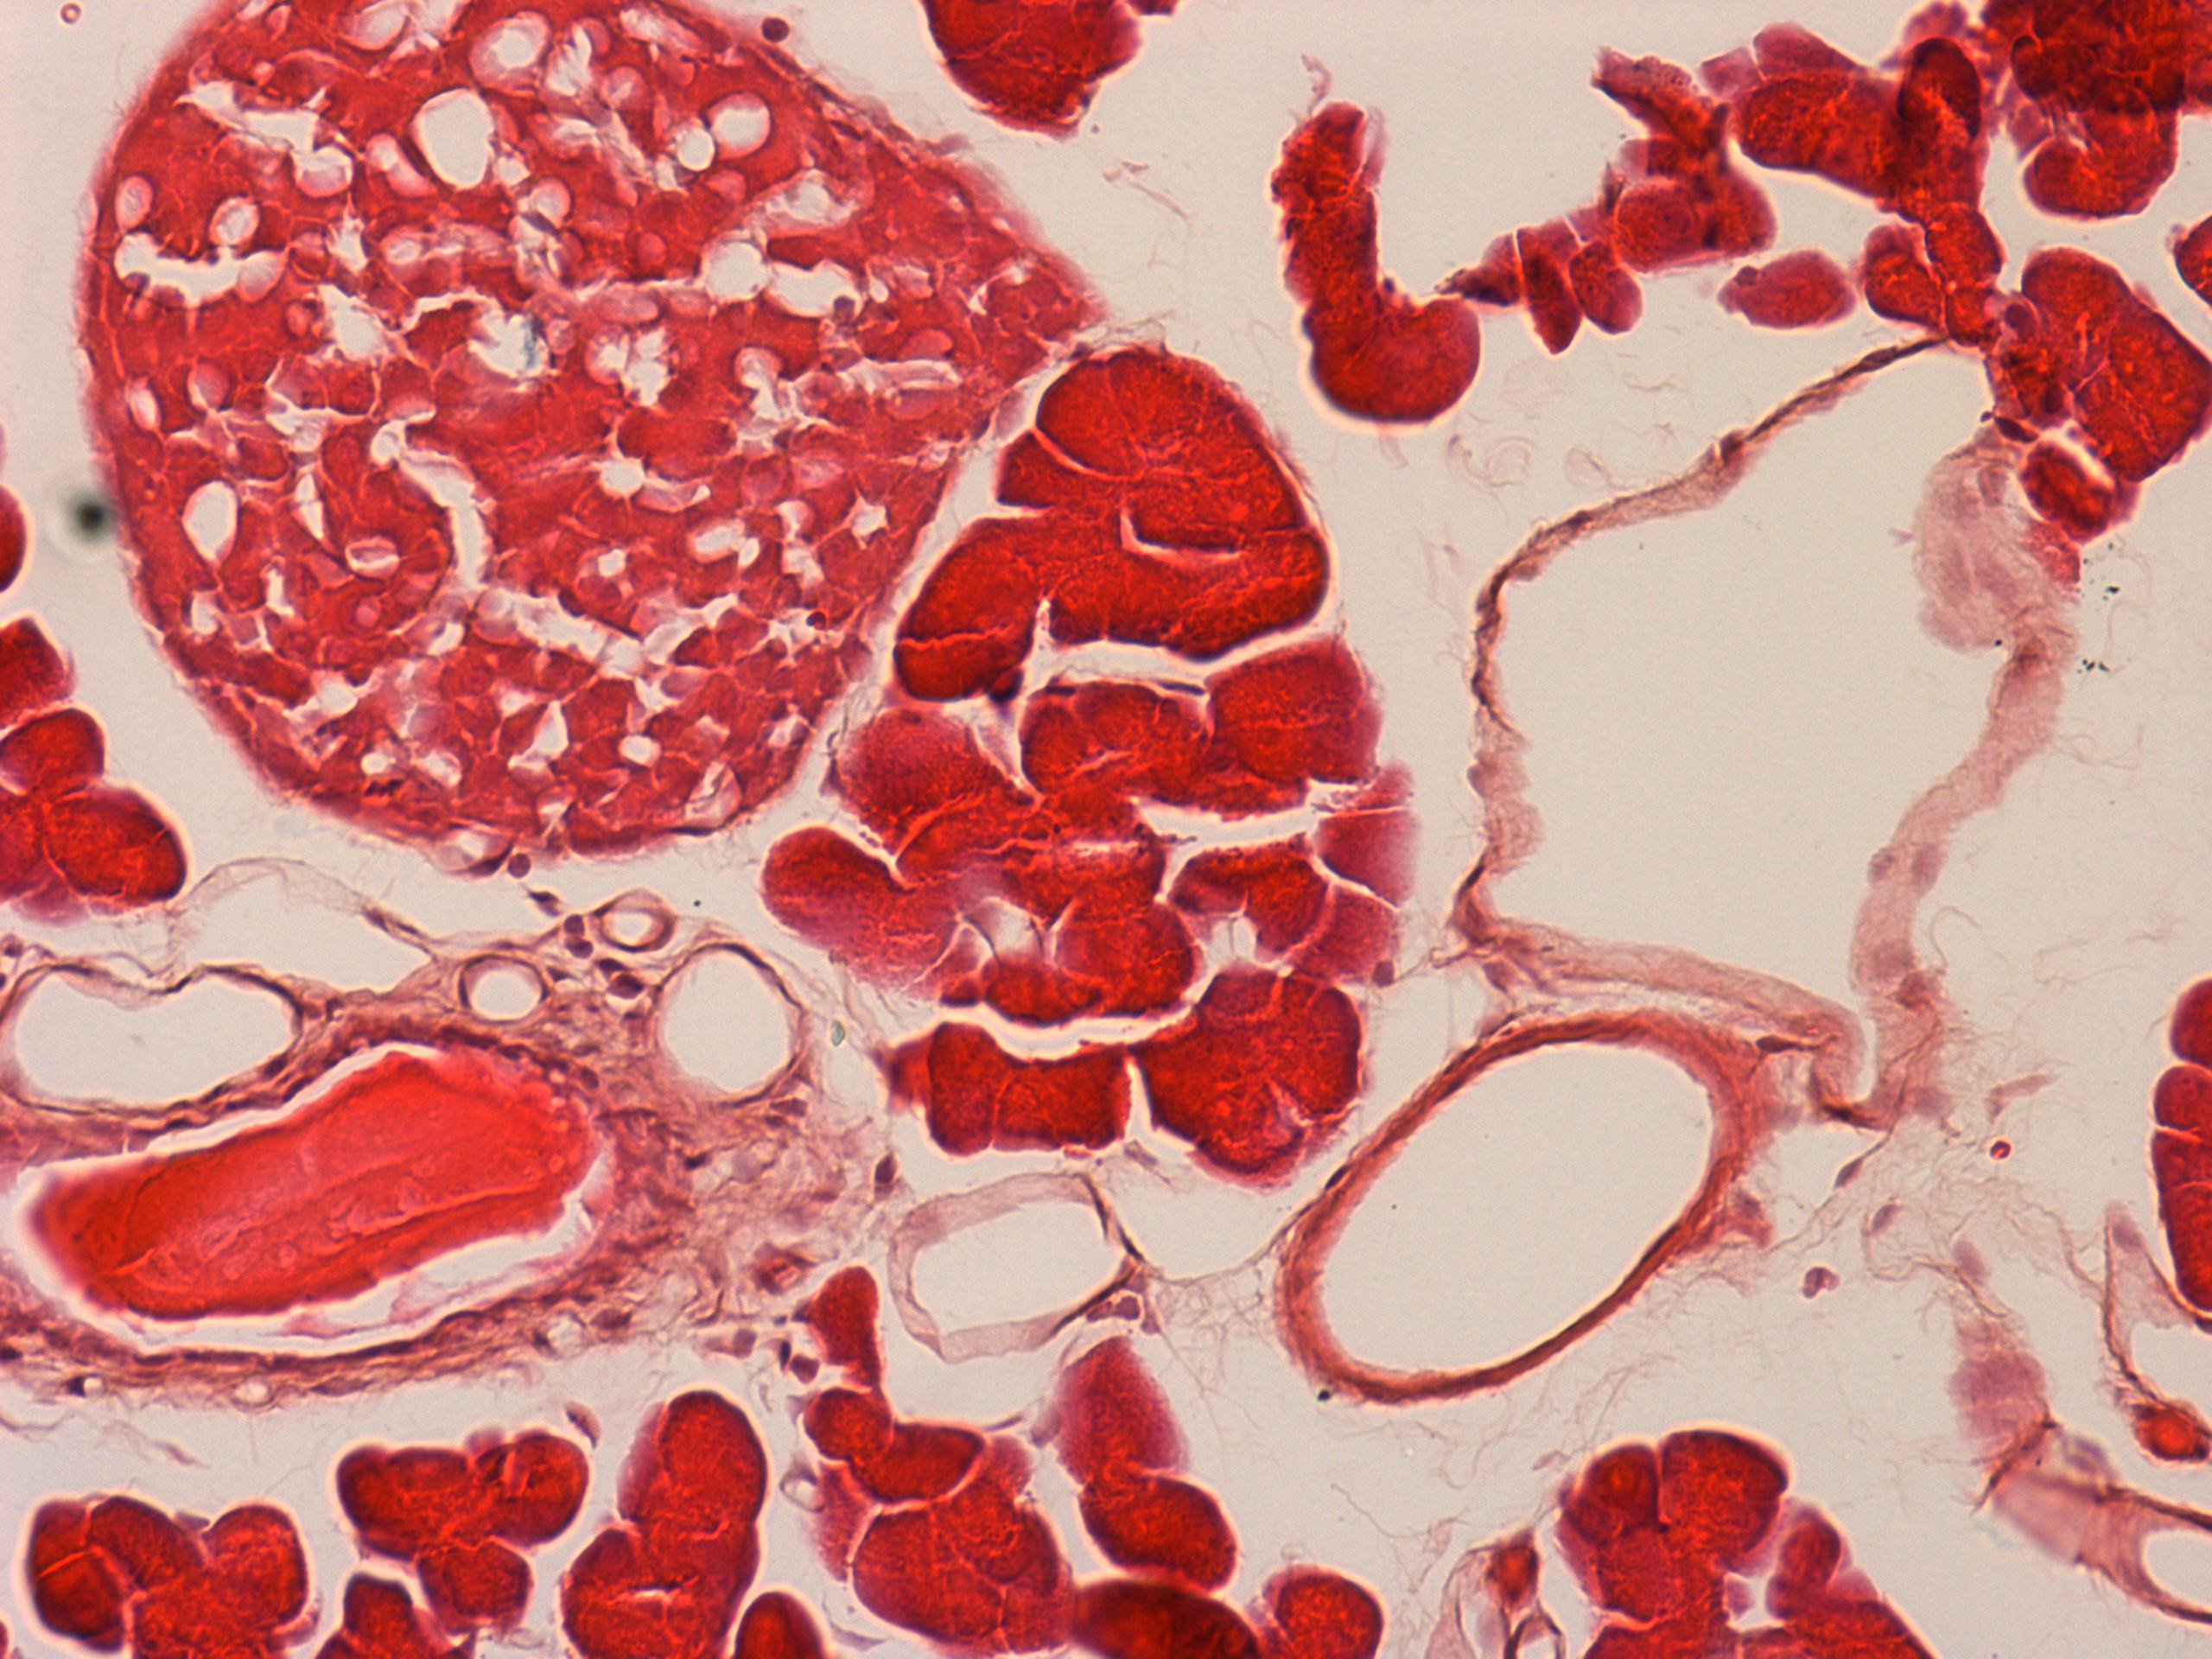
\includegraphics[width=86.2mm]{image/HE-20x-2.jpg}
    \end{center}
    \psset{unit=2mm}
    \begin{pspicture}(-0.5,-1.5)(19.5,-1.5)
        \psaxes[ticks=x,tickstyle=top,Dx= 1,ticksize=1.5mm,labels=none](0,0)(20,0)
        \psaxes[ticks=x,tickstyle=top,Dx= 5,ticksize=2.5mm            ](0,0)(20,0)
        \psaxes[ticks=x,tickstyle=top,Dx=10,ticksize=3.5mm,labels=none](0,0)(20,0)
    \end{pspicture}
    \caption{H\&E 200x}
    \label{red-1}
\end{figure}

\begin{figure}
    \begin{center}
        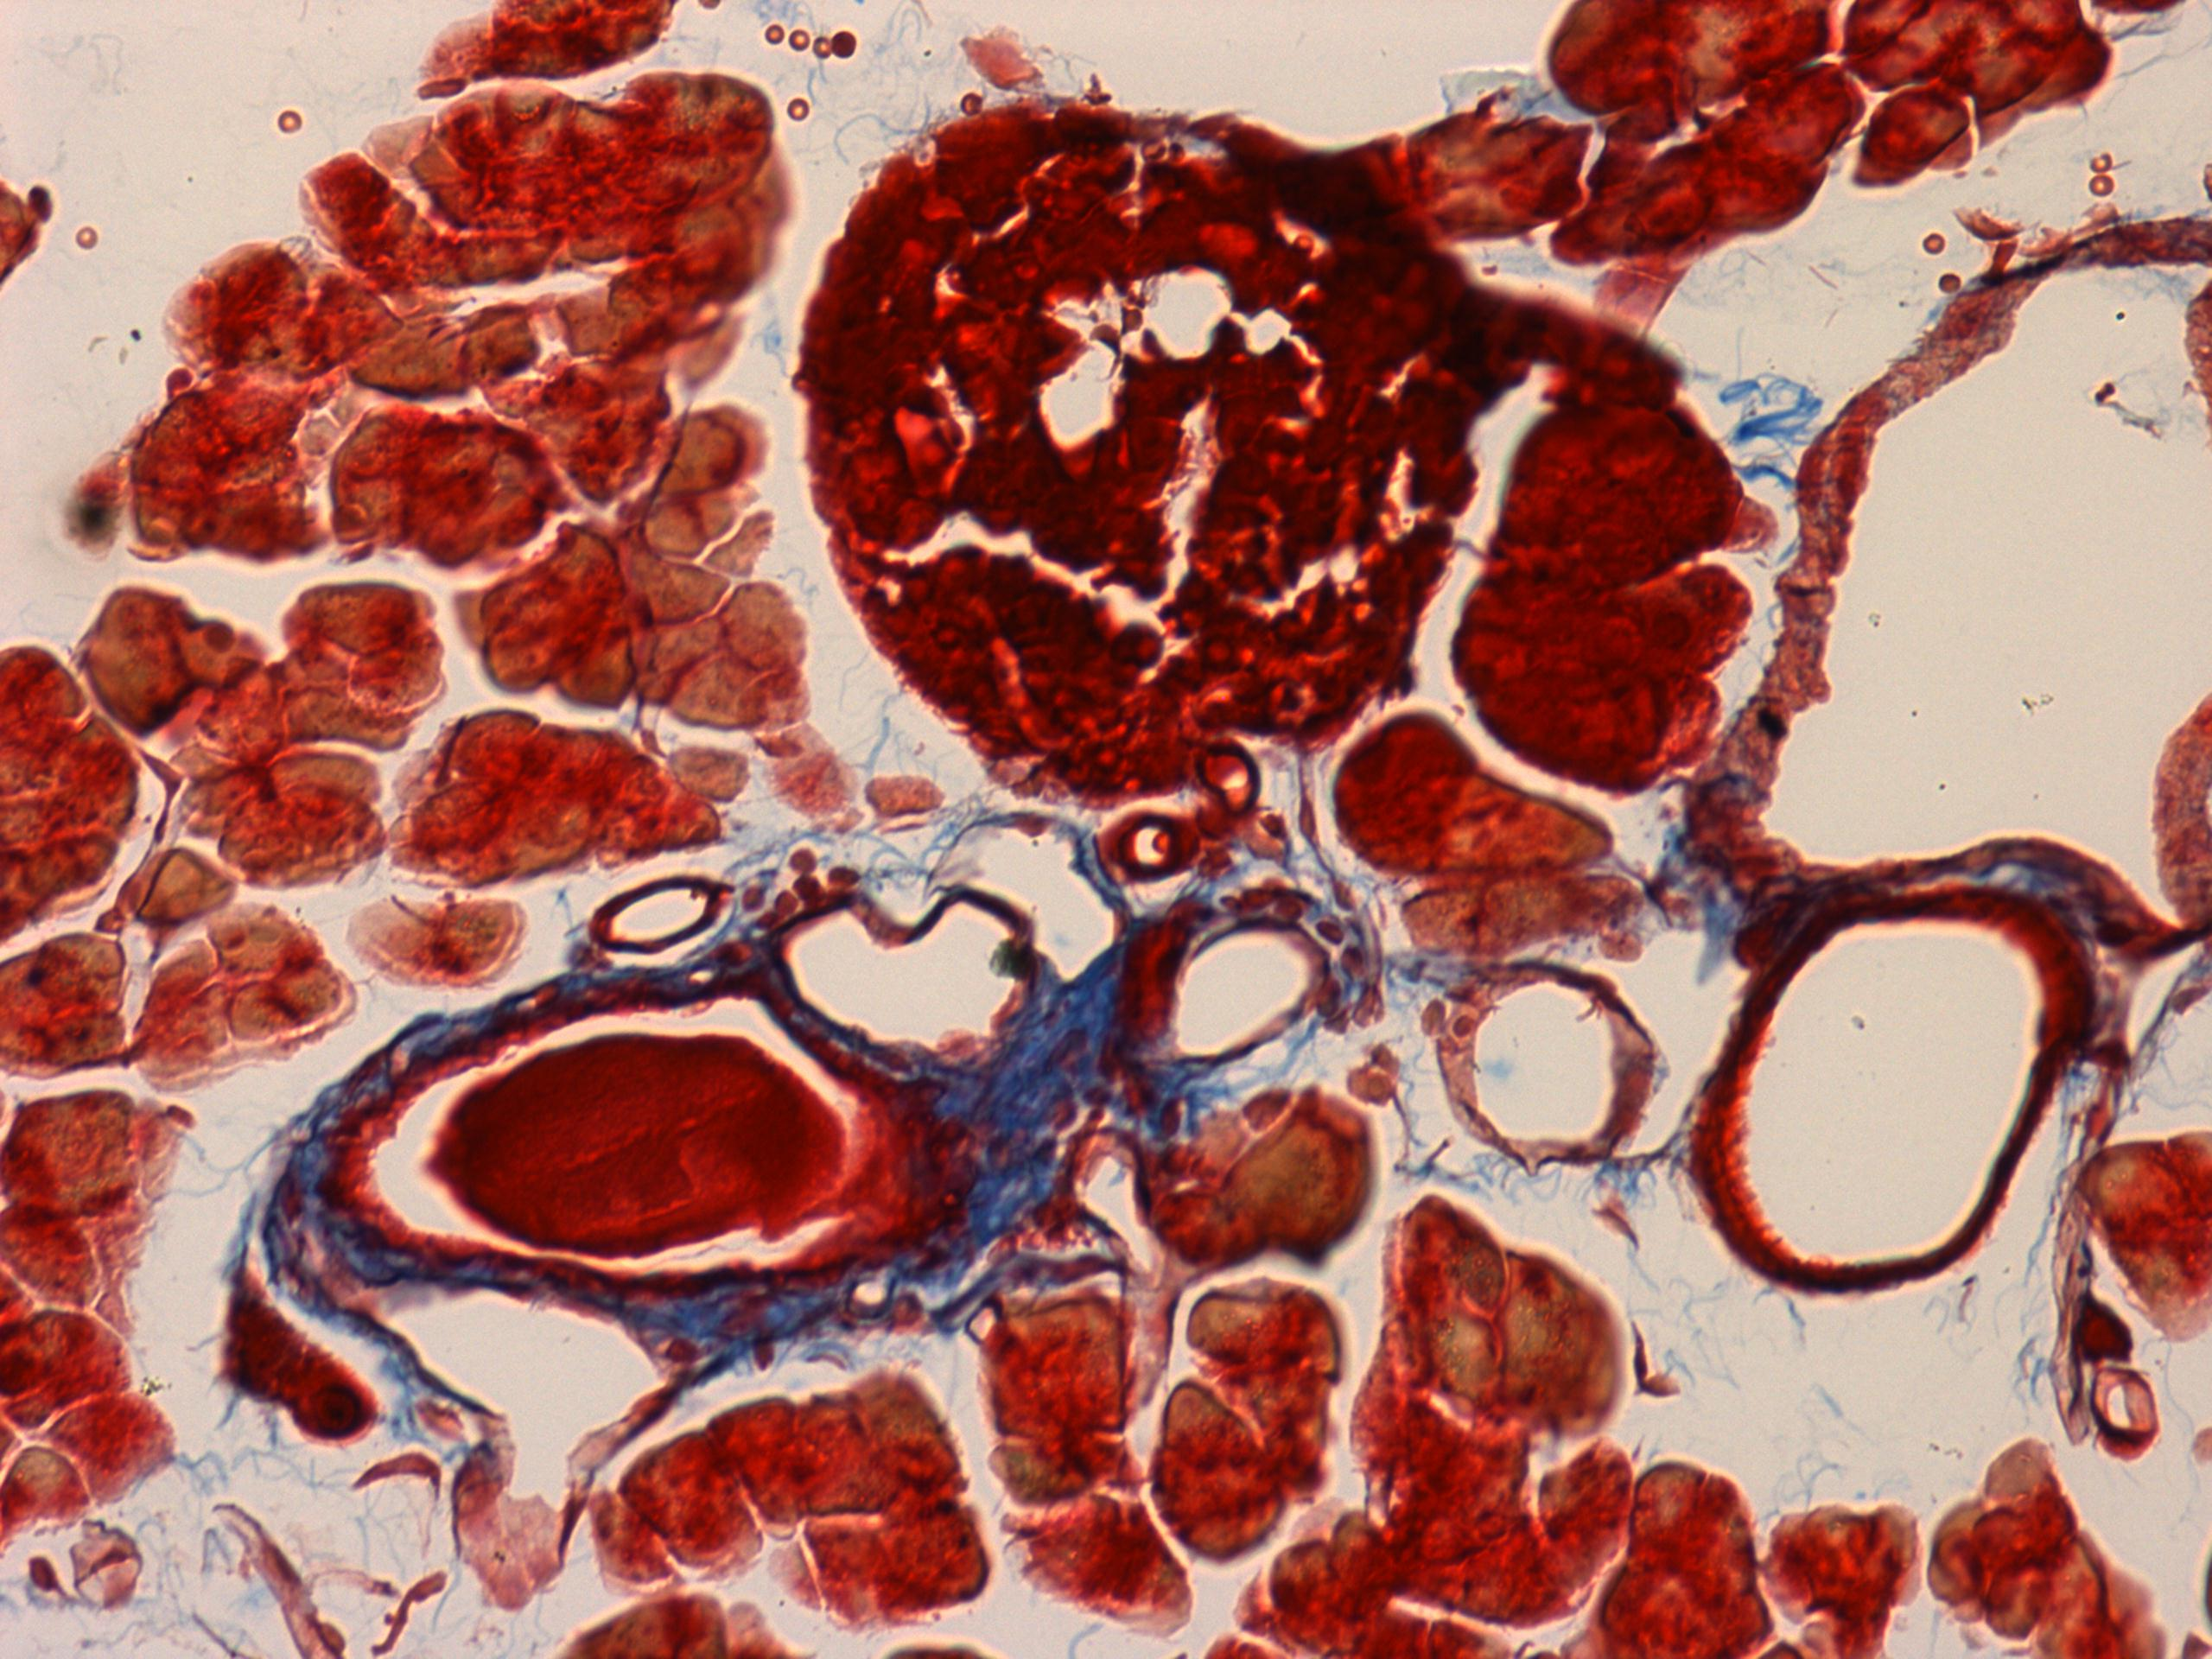
\includegraphics[width=86.2mm]{image/Tri-20x-2.jpg}
    \end{center}
    \psset{unit=2mm}
    \begin{pspicture}(-0.5,-1.5)(19.5,-1.5)
        \psaxes[ticks=x,tickstyle=top,Dx= 1,ticksize=1.5mm,labels=none](0,0)(20,0)
        \psaxes[ticks=x,tickstyle=top,Dx= 5,ticksize=2.5mm            ](0,0)(20,0)
        \psaxes[ticks=x,tickstyle=top,Dx=10,ticksize=3.5mm,labels=none](0,0)(20,0)
    \end{pspicture}
    \caption{Masson's trichrome 200x}
\end{figure}

\begin{figure}
    \begin{center}
        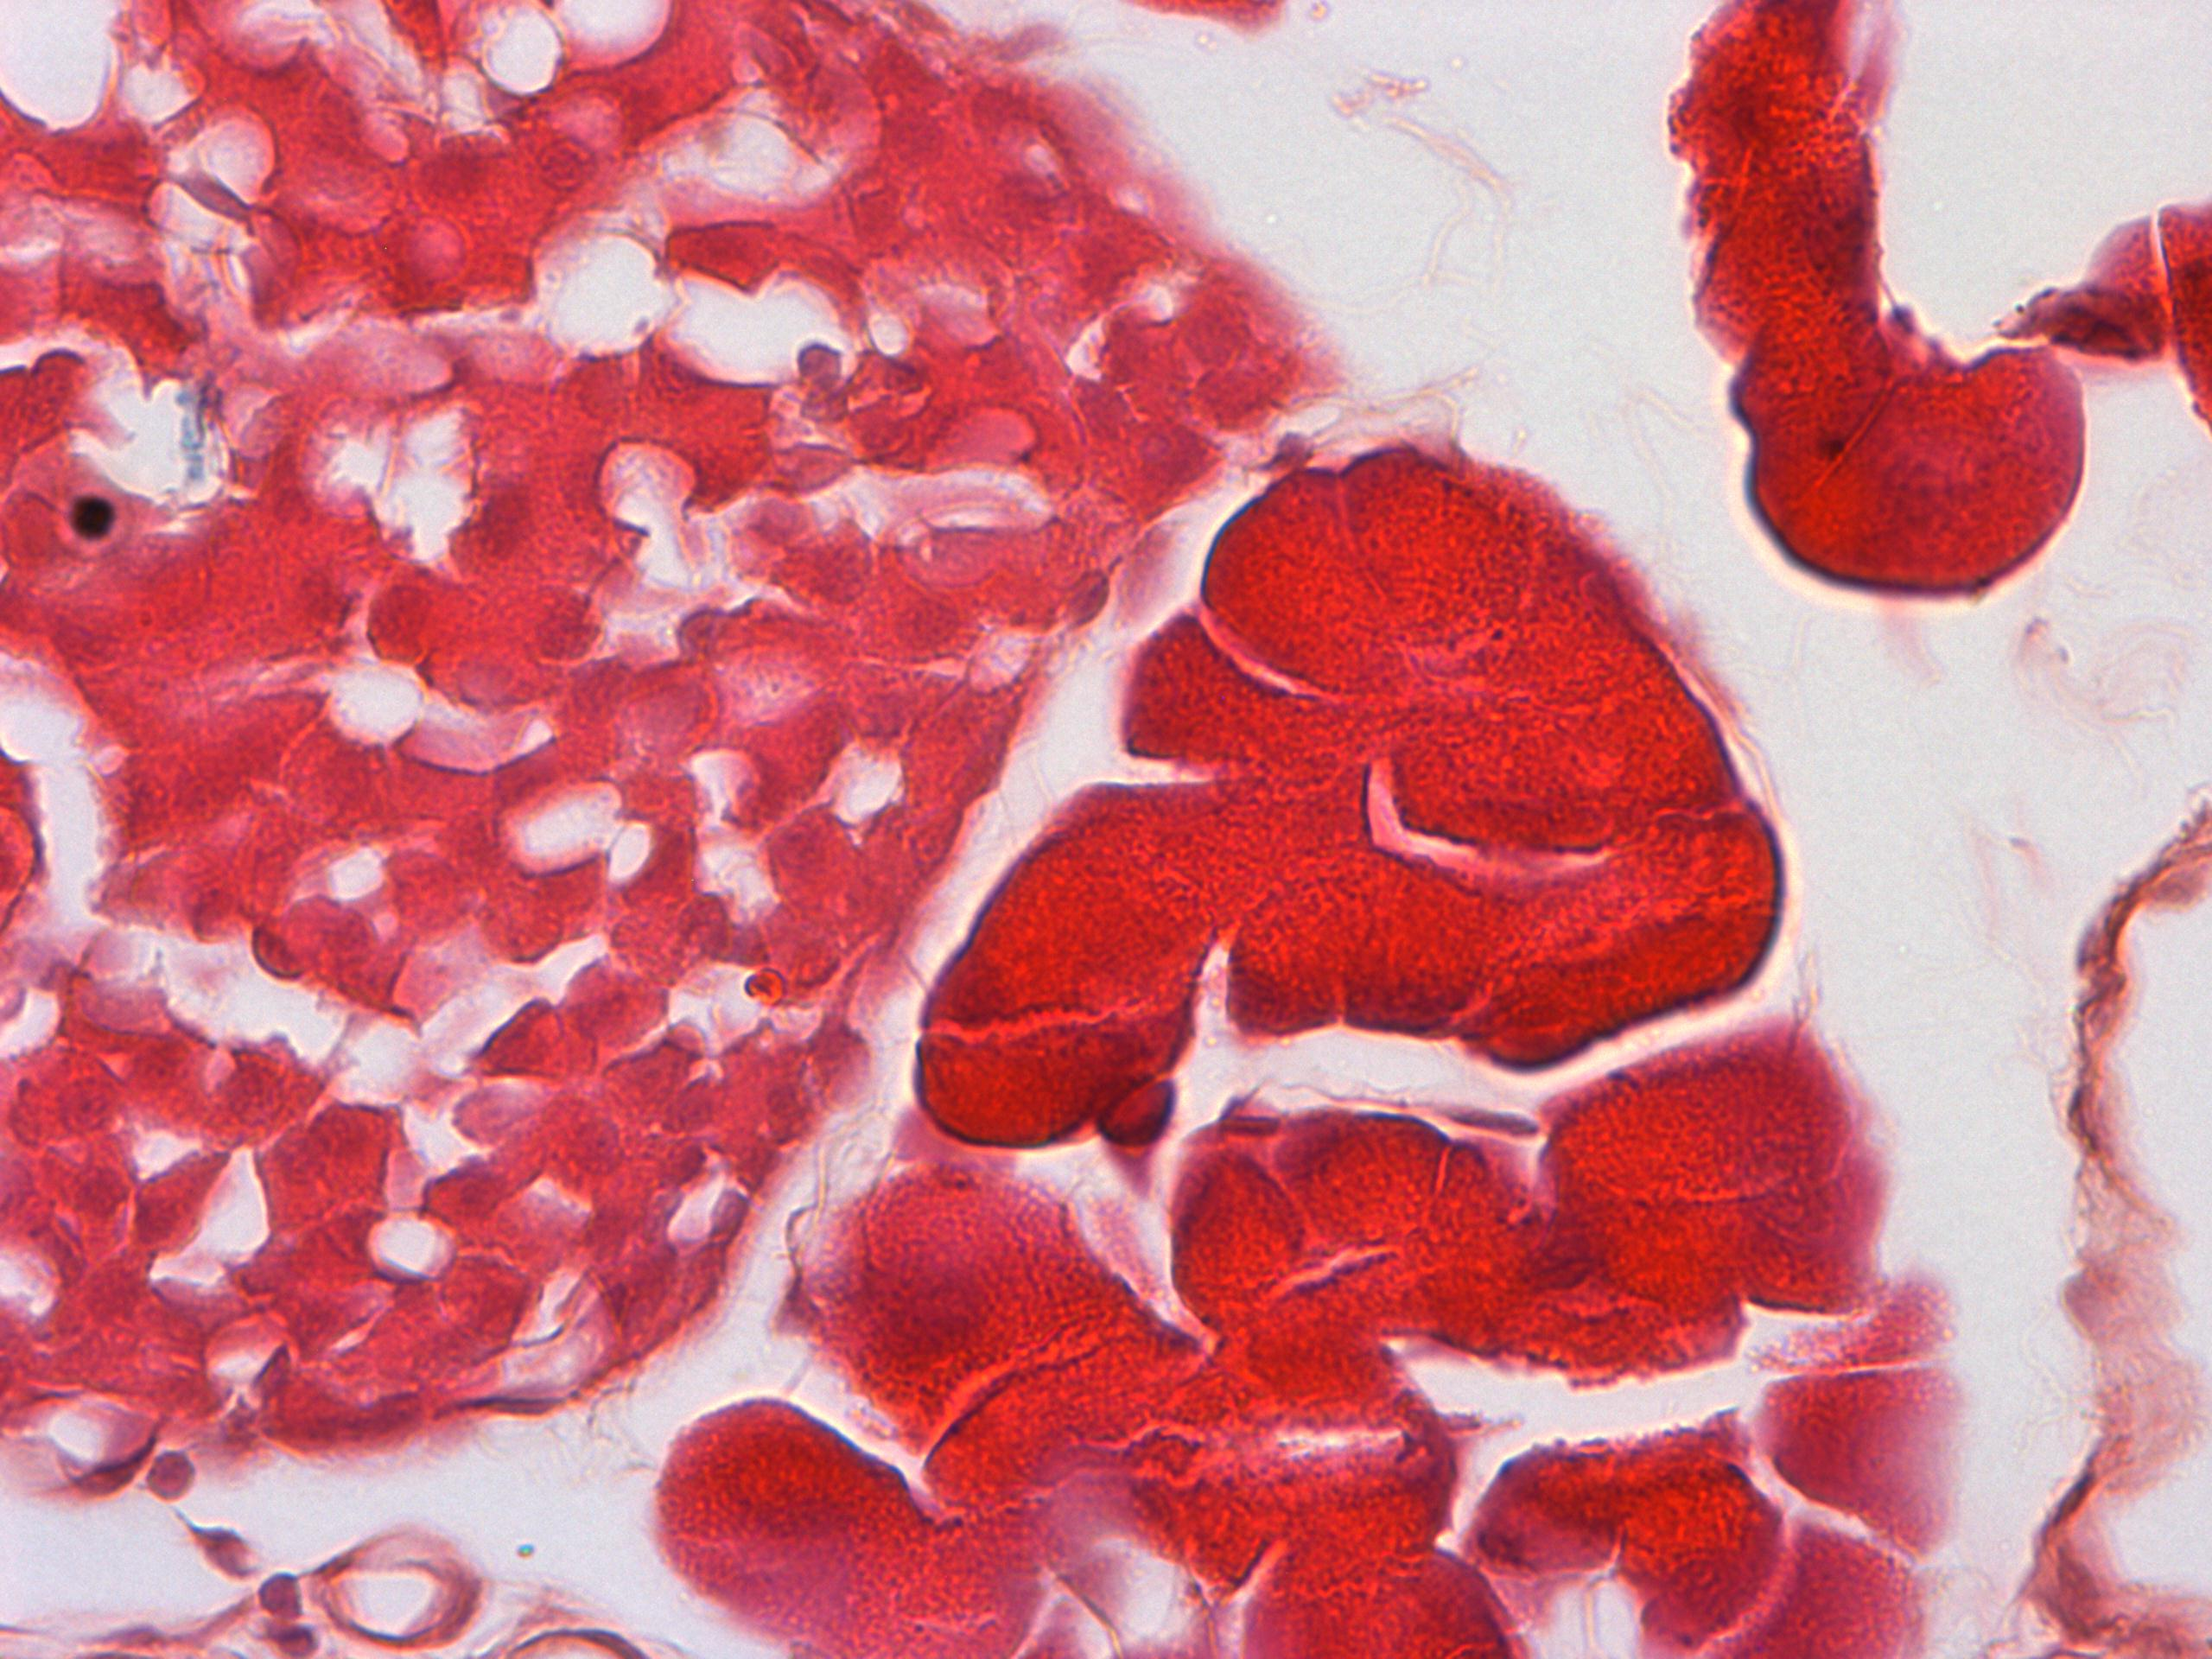
\includegraphics[width=86.2mm]{image/HE-40x-1.jpg}
    \end{center}
    \psset{unit=4mm}
    \begin{pspicture}(-0.25,-0.75)(9.75,-0.75)
        \psaxes[ticks=x,tickstyle=top,Dx= 1,ticksize=1.5mm,labels=none](0,0)(10,0)
        \psaxes[ticks=x,tickstyle=top,Dx= 5,ticksize=2.5mm            ](0,0)(10,0)
        \psaxes[ticks=x,tickstyle=top,Dx=10,ticksize=3.5mm,labels=none](0,0)(10,0)
    \end{pspicture}
    \caption{H\&E 400x 之一}
    \label{red-2}
\end{figure}

\begin{figure}
    \begin{center}
        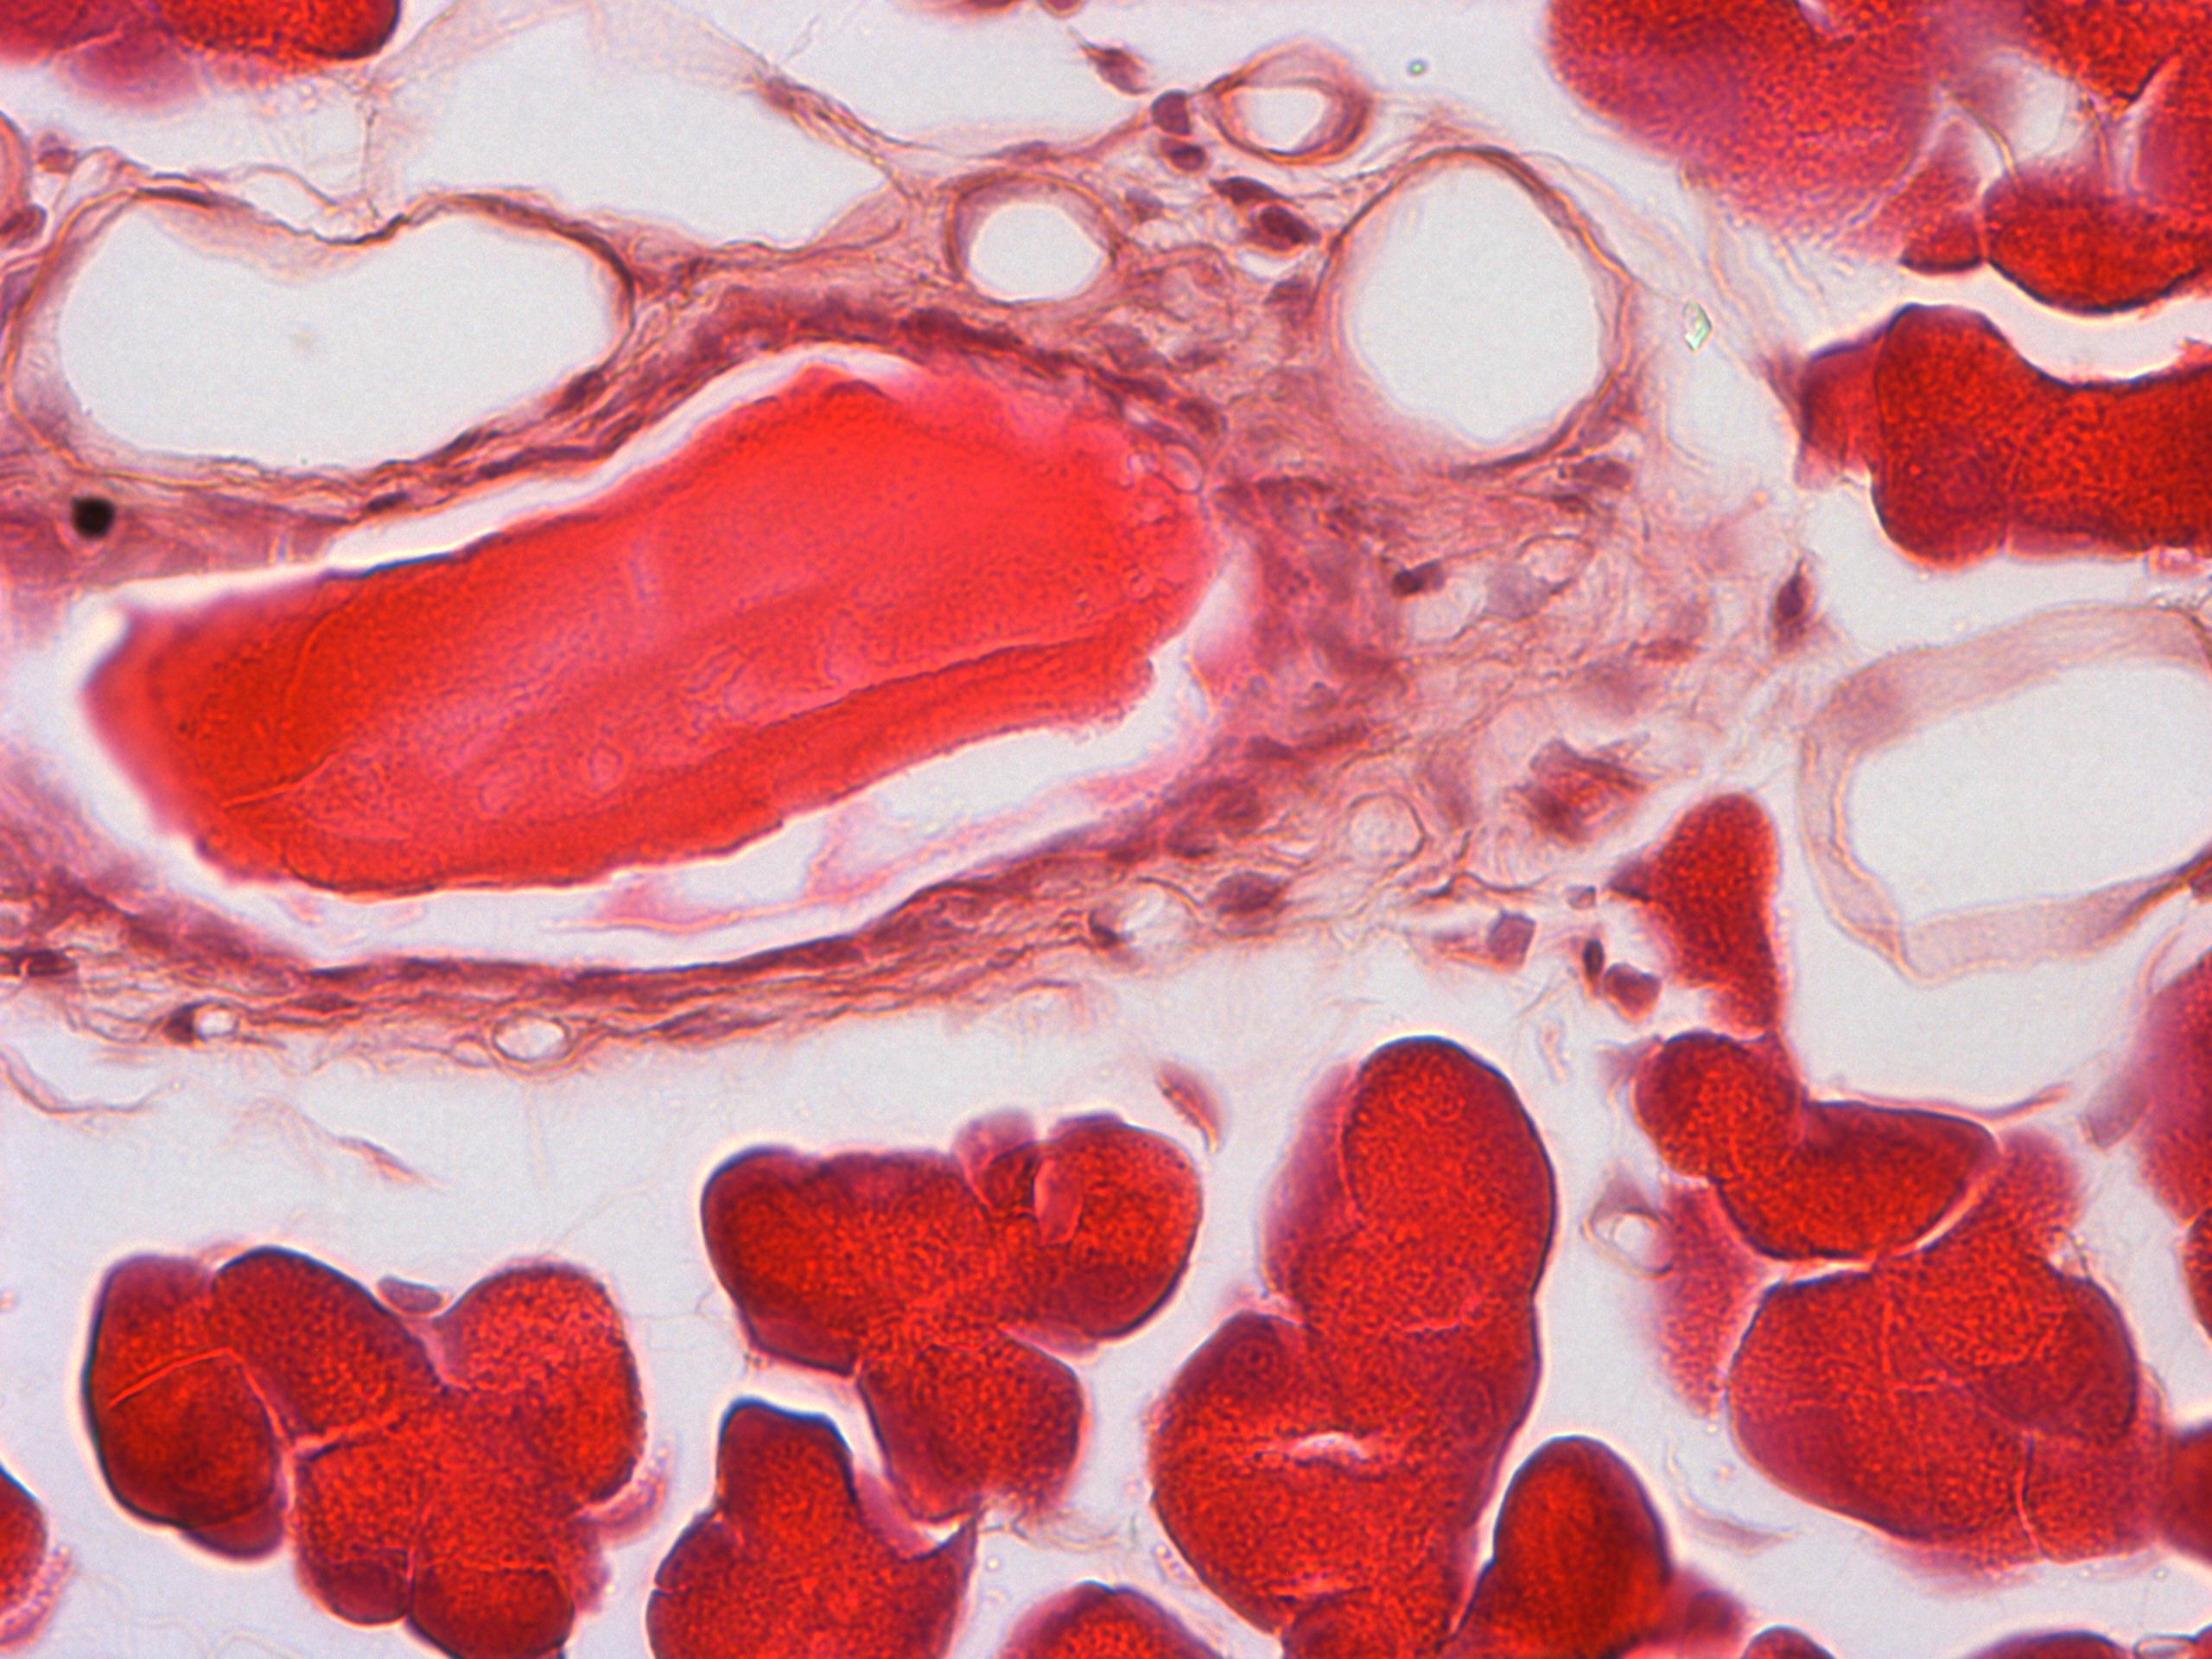
\includegraphics[width=86.2mm]{image/HE-40x-2.jpg}
    \end{center}
    \psset{unit=4mm}
    \begin{pspicture}(-0.25,-0.75)(9.75,-0.75)
        \psaxes[ticks=x,tickstyle=top,Dx= 1,ticksize=1.5mm,labels=none](0,0)(10,0)
        \psaxes[ticks=x,tickstyle=top,Dx= 5,ticksize=2.5mm            ](0,0)(10,0)
        \psaxes[ticks=x,tickstyle=top,Dx=10,ticksize=3.5mm,labels=none](0,0)(10,0)
    \end{pspicture}
    \caption{H\&E 400x 之二}
    \label{blue-1}
\end{figure}

\begin{figure}
    \begin{center}
        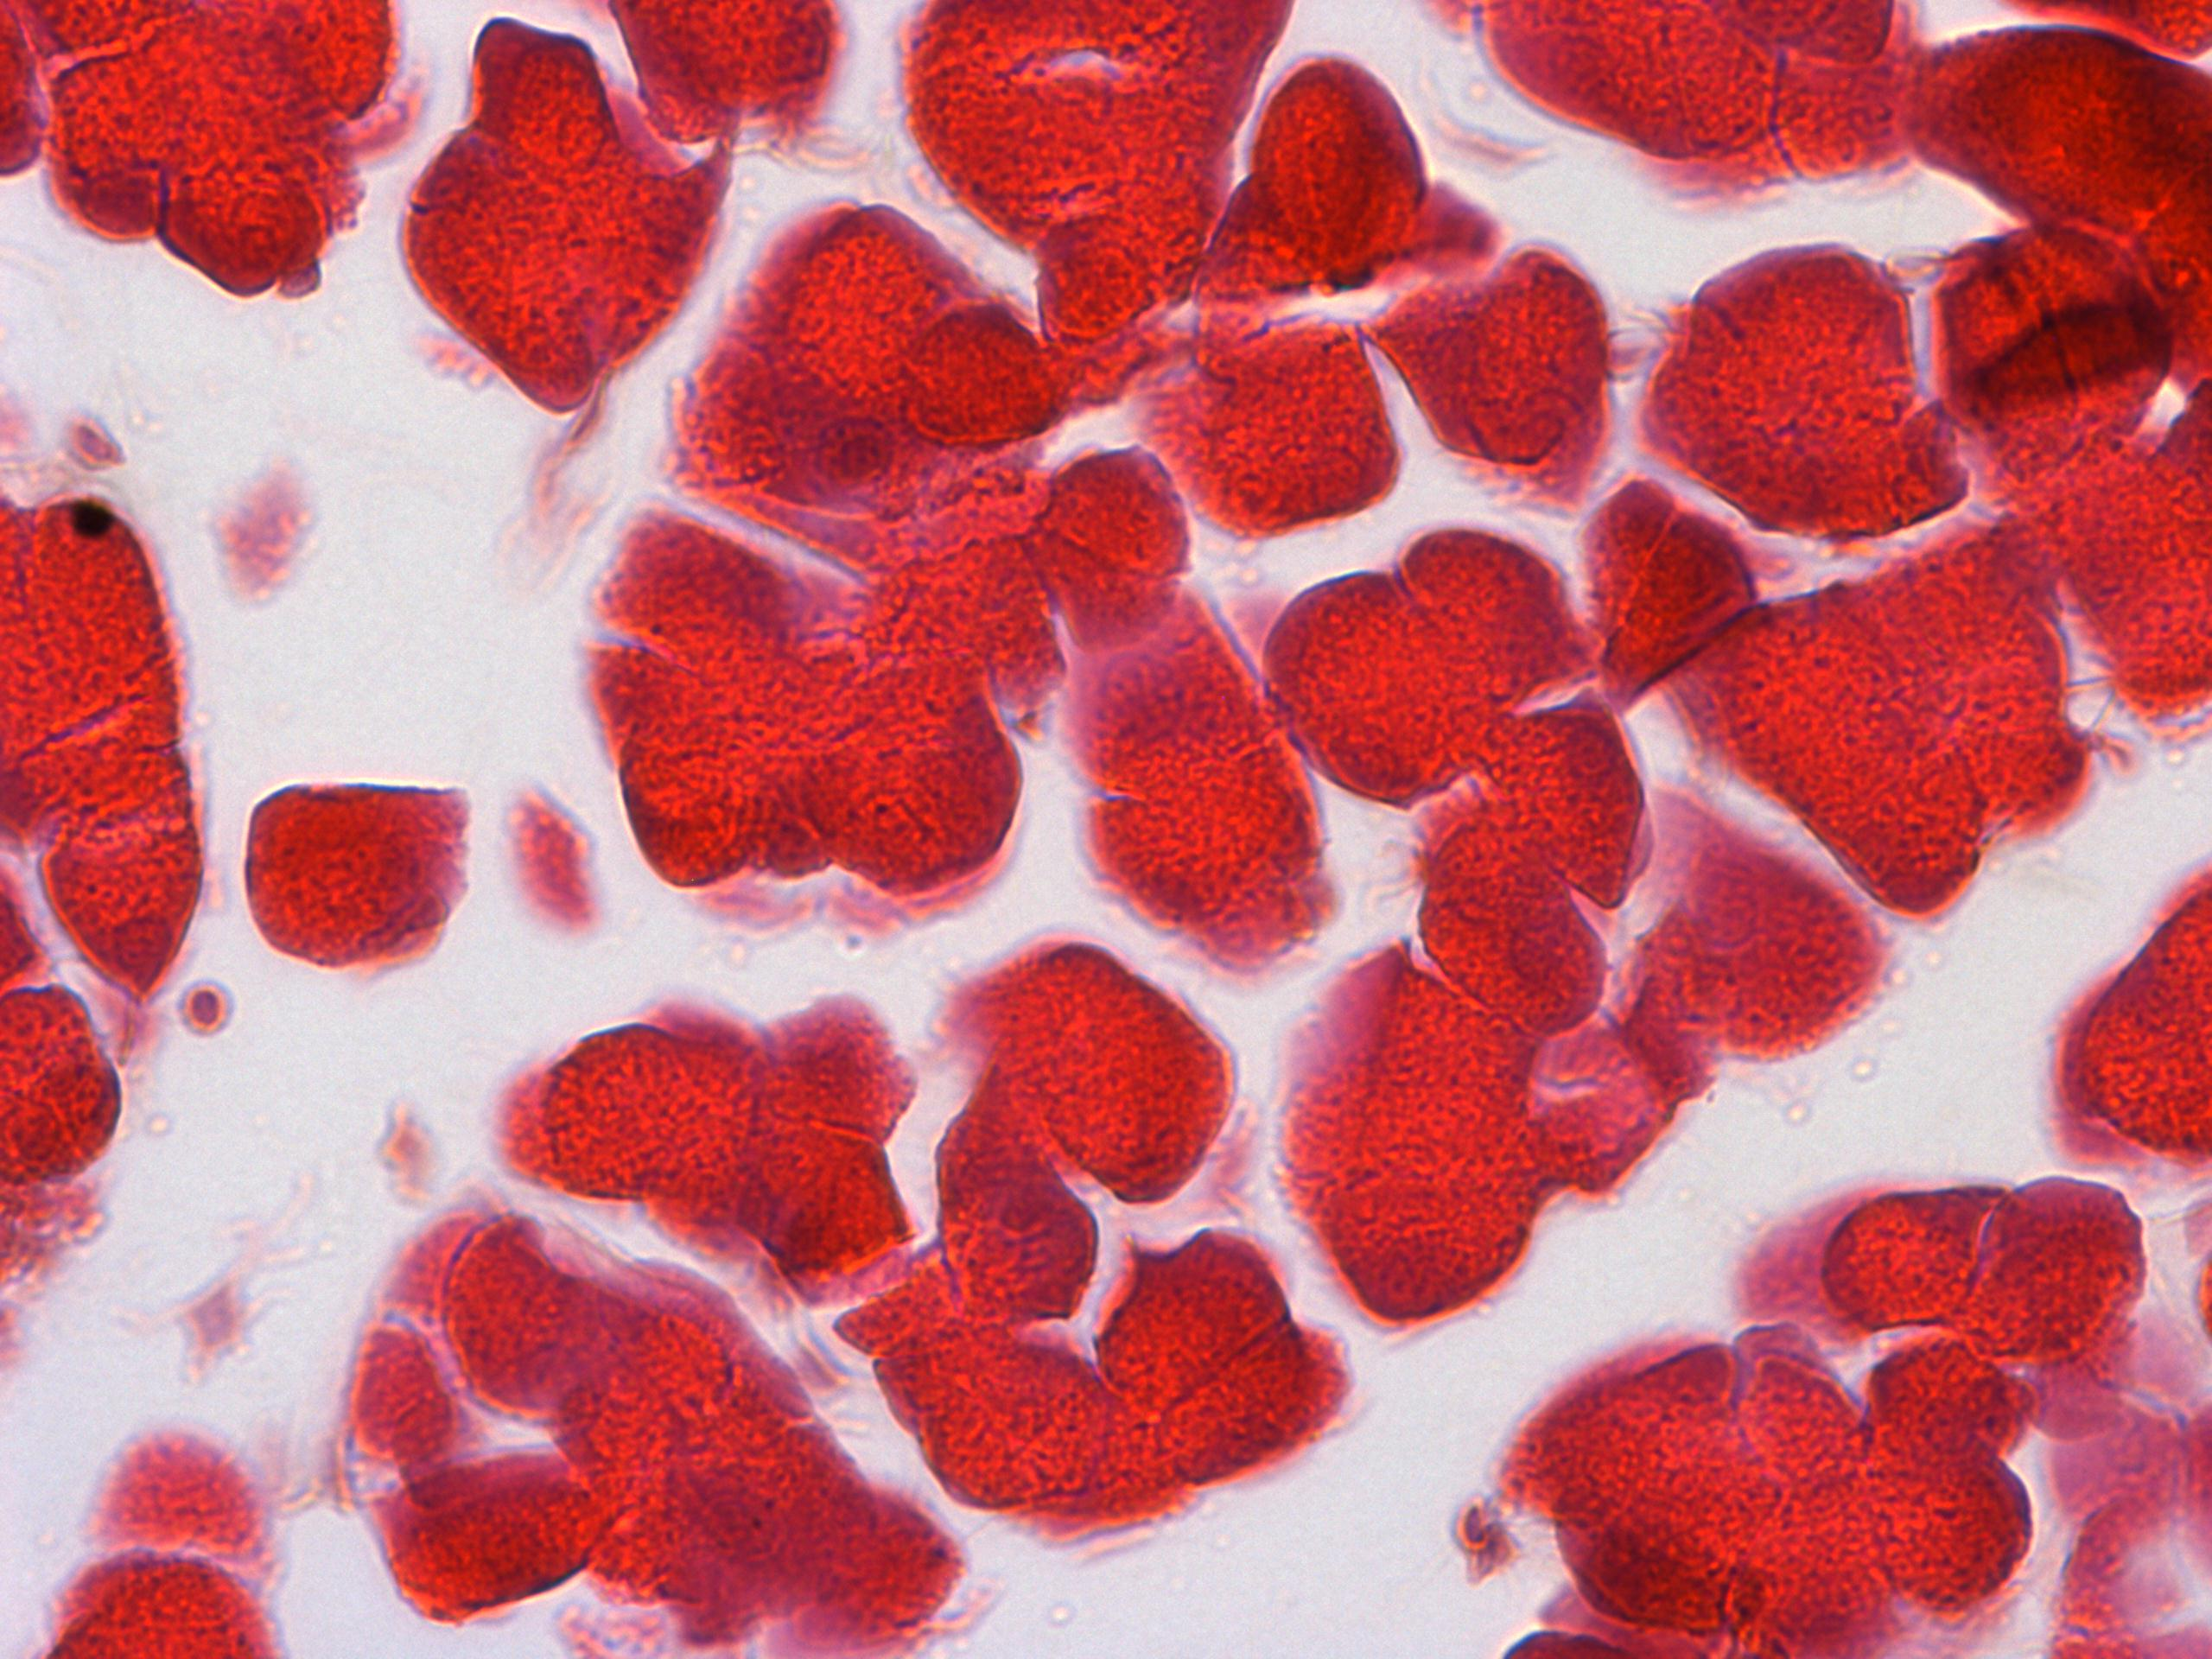
\includegraphics[width=86.2mm]{image/HE-40x-3.jpg}
    \end{center}
    \psset{unit=4mm}
    \begin{pspicture}(-0.25,-0.75)(9.75,-0.75)
        \psaxes[ticks=x,tickstyle=top,Dx= 1,ticksize=1.5mm,labels=none](0,0)(10,0)
        \psaxes[ticks=x,tickstyle=top,Dx= 5,ticksize=2.5mm            ](0,0)(10,0)
        \psaxes[ticks=x,tickstyle=top,Dx=10,ticksize=3.5mm,labels=none](0,0)(10,0)
    \end{pspicture}
    \caption{H\&E 400x 之三}
\end{figure}

\begin{figure}
    \begin{center}
        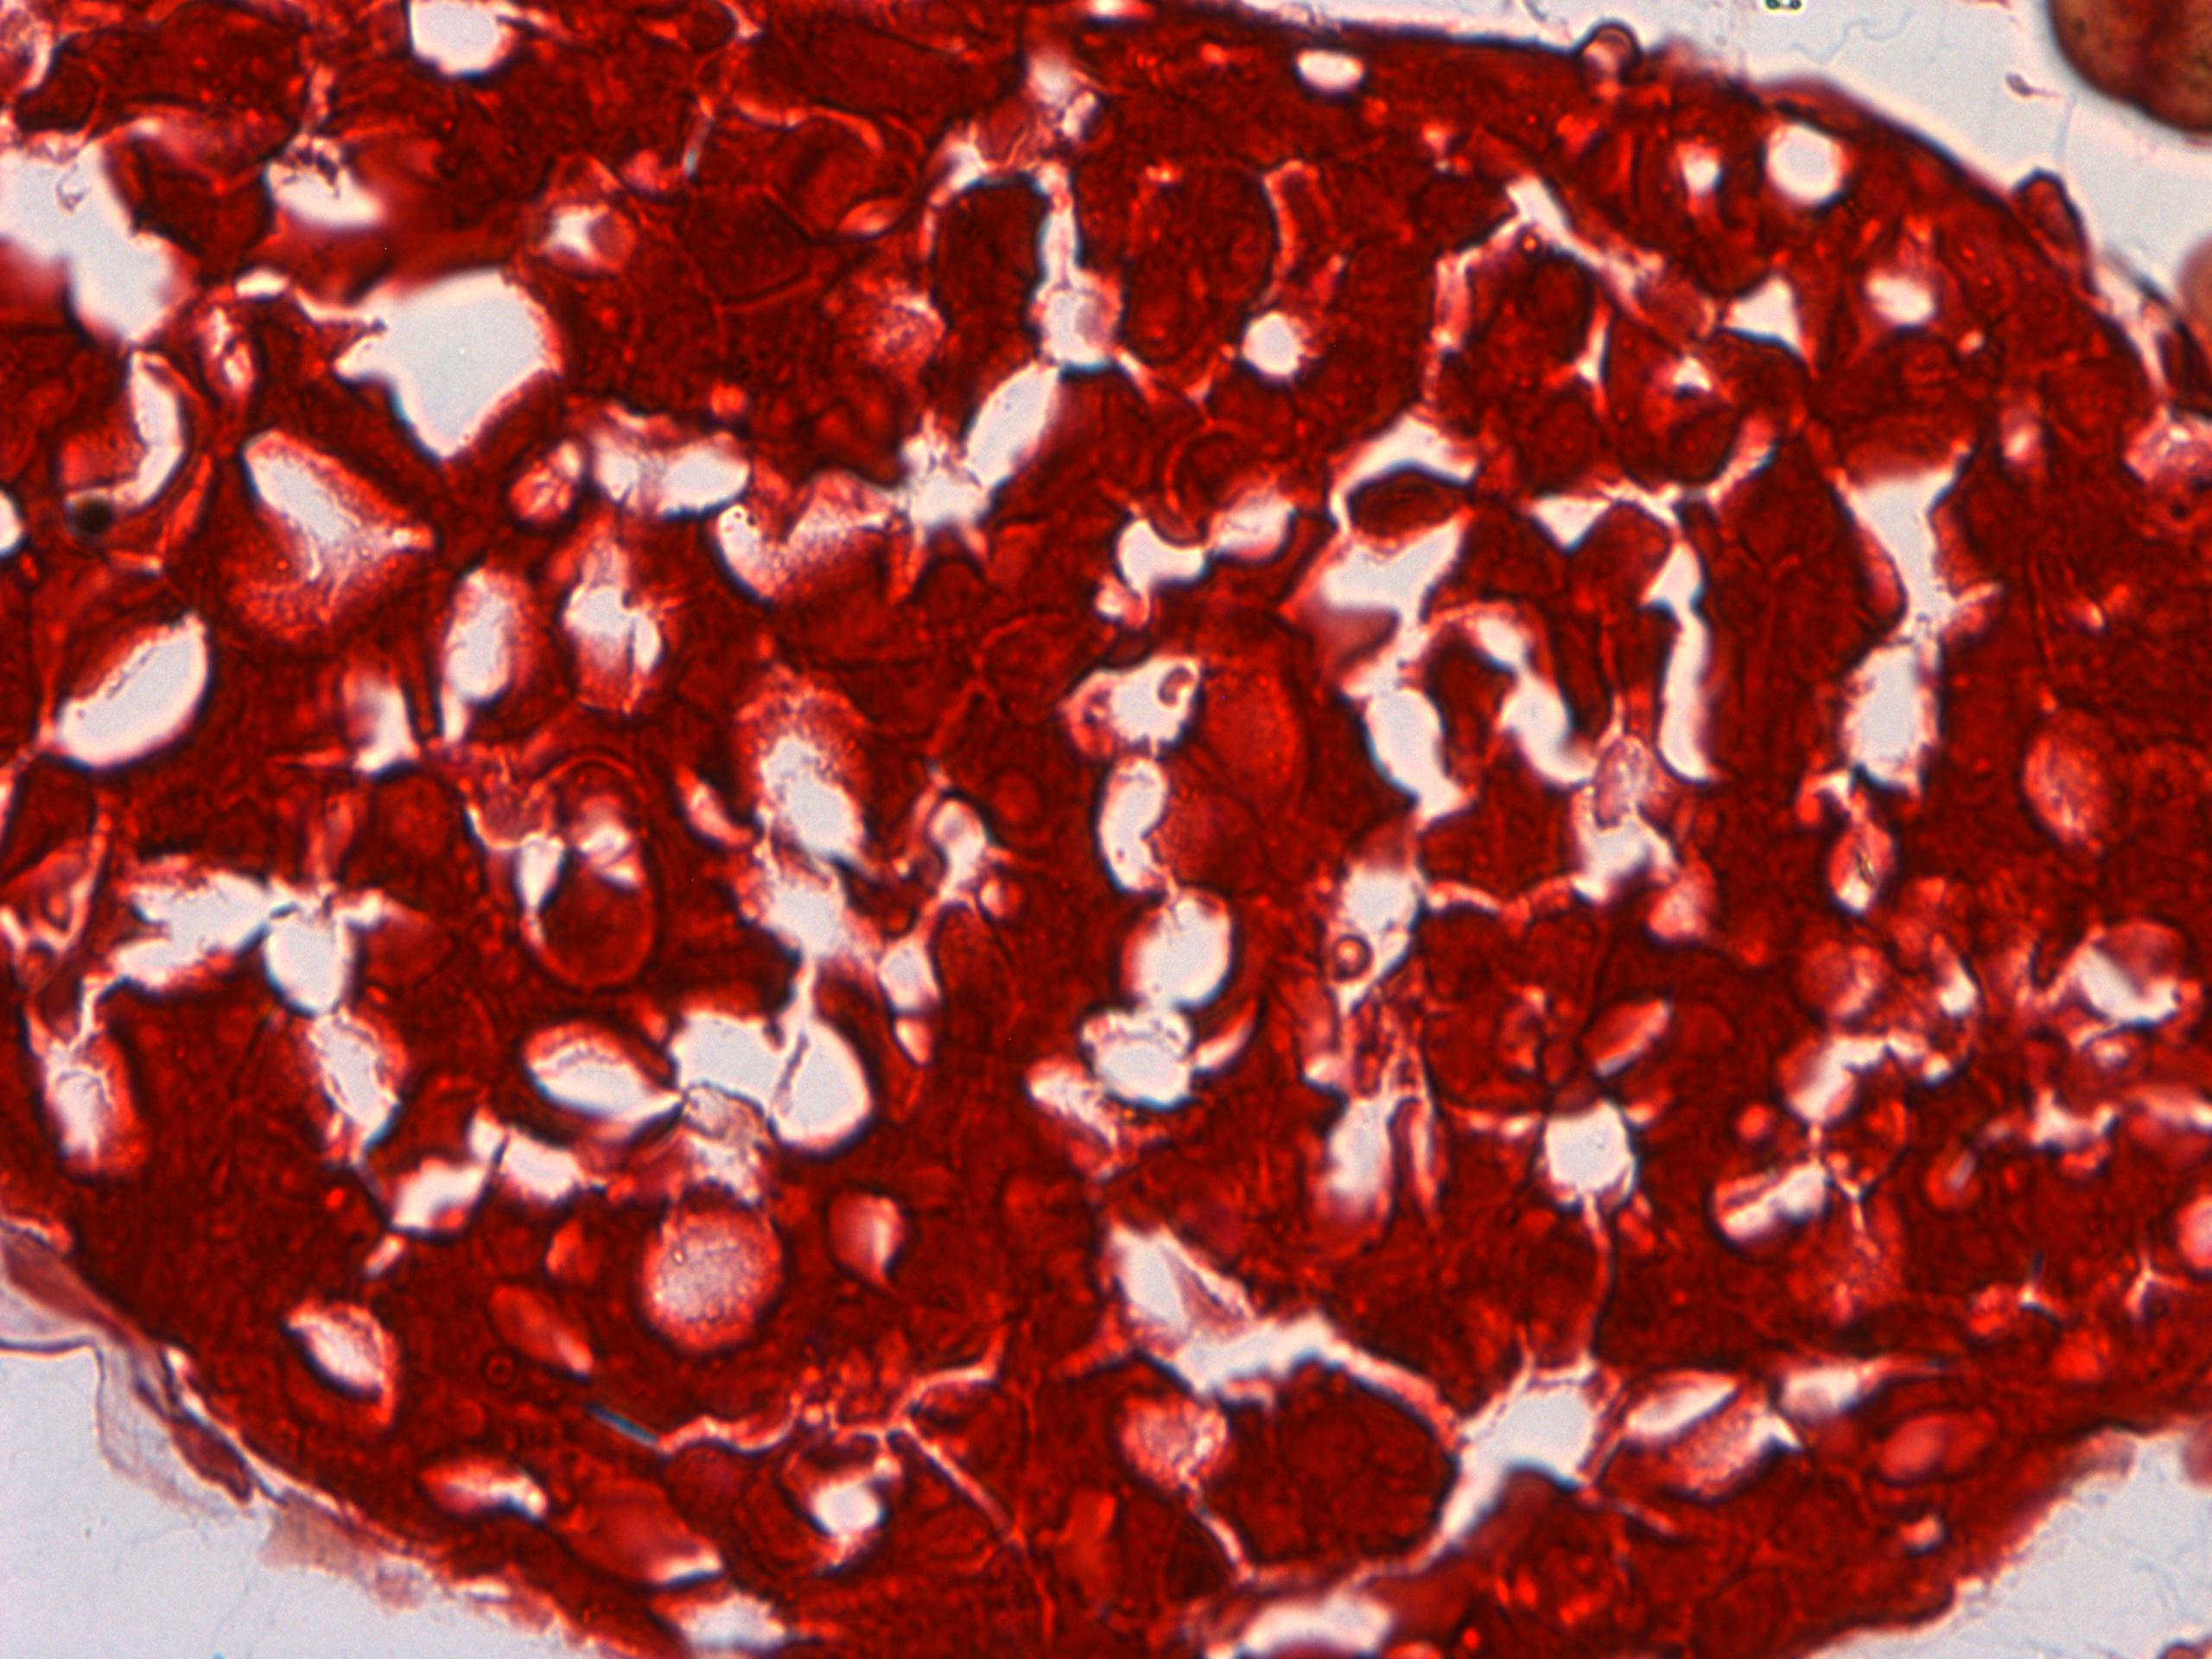
\includegraphics[width=86.2mm]{image/Tri-40x-1.jpg}
    \end{center}
    \psset{unit=4mm}
    \begin{pspicture}(-0.25,-0.75)(9.75,-0.75)
        \psaxes[ticks=x,tickstyle=top,Dx= 1,ticksize=1.5mm,labels=none](0,0)(10,0)
        \psaxes[ticks=x,tickstyle=top,Dx= 5,ticksize=2.5mm            ](0,0)(10,0)
        \psaxes[ticks=x,tickstyle=top,Dx=10,ticksize=3.5mm,labels=none](0,0)(10,0)
    \end{pspicture}
    \caption{Masson's trichrome 400x 之一}
    \label{red-3}
\end{figure}

\begin{figure}
    \begin{center}
        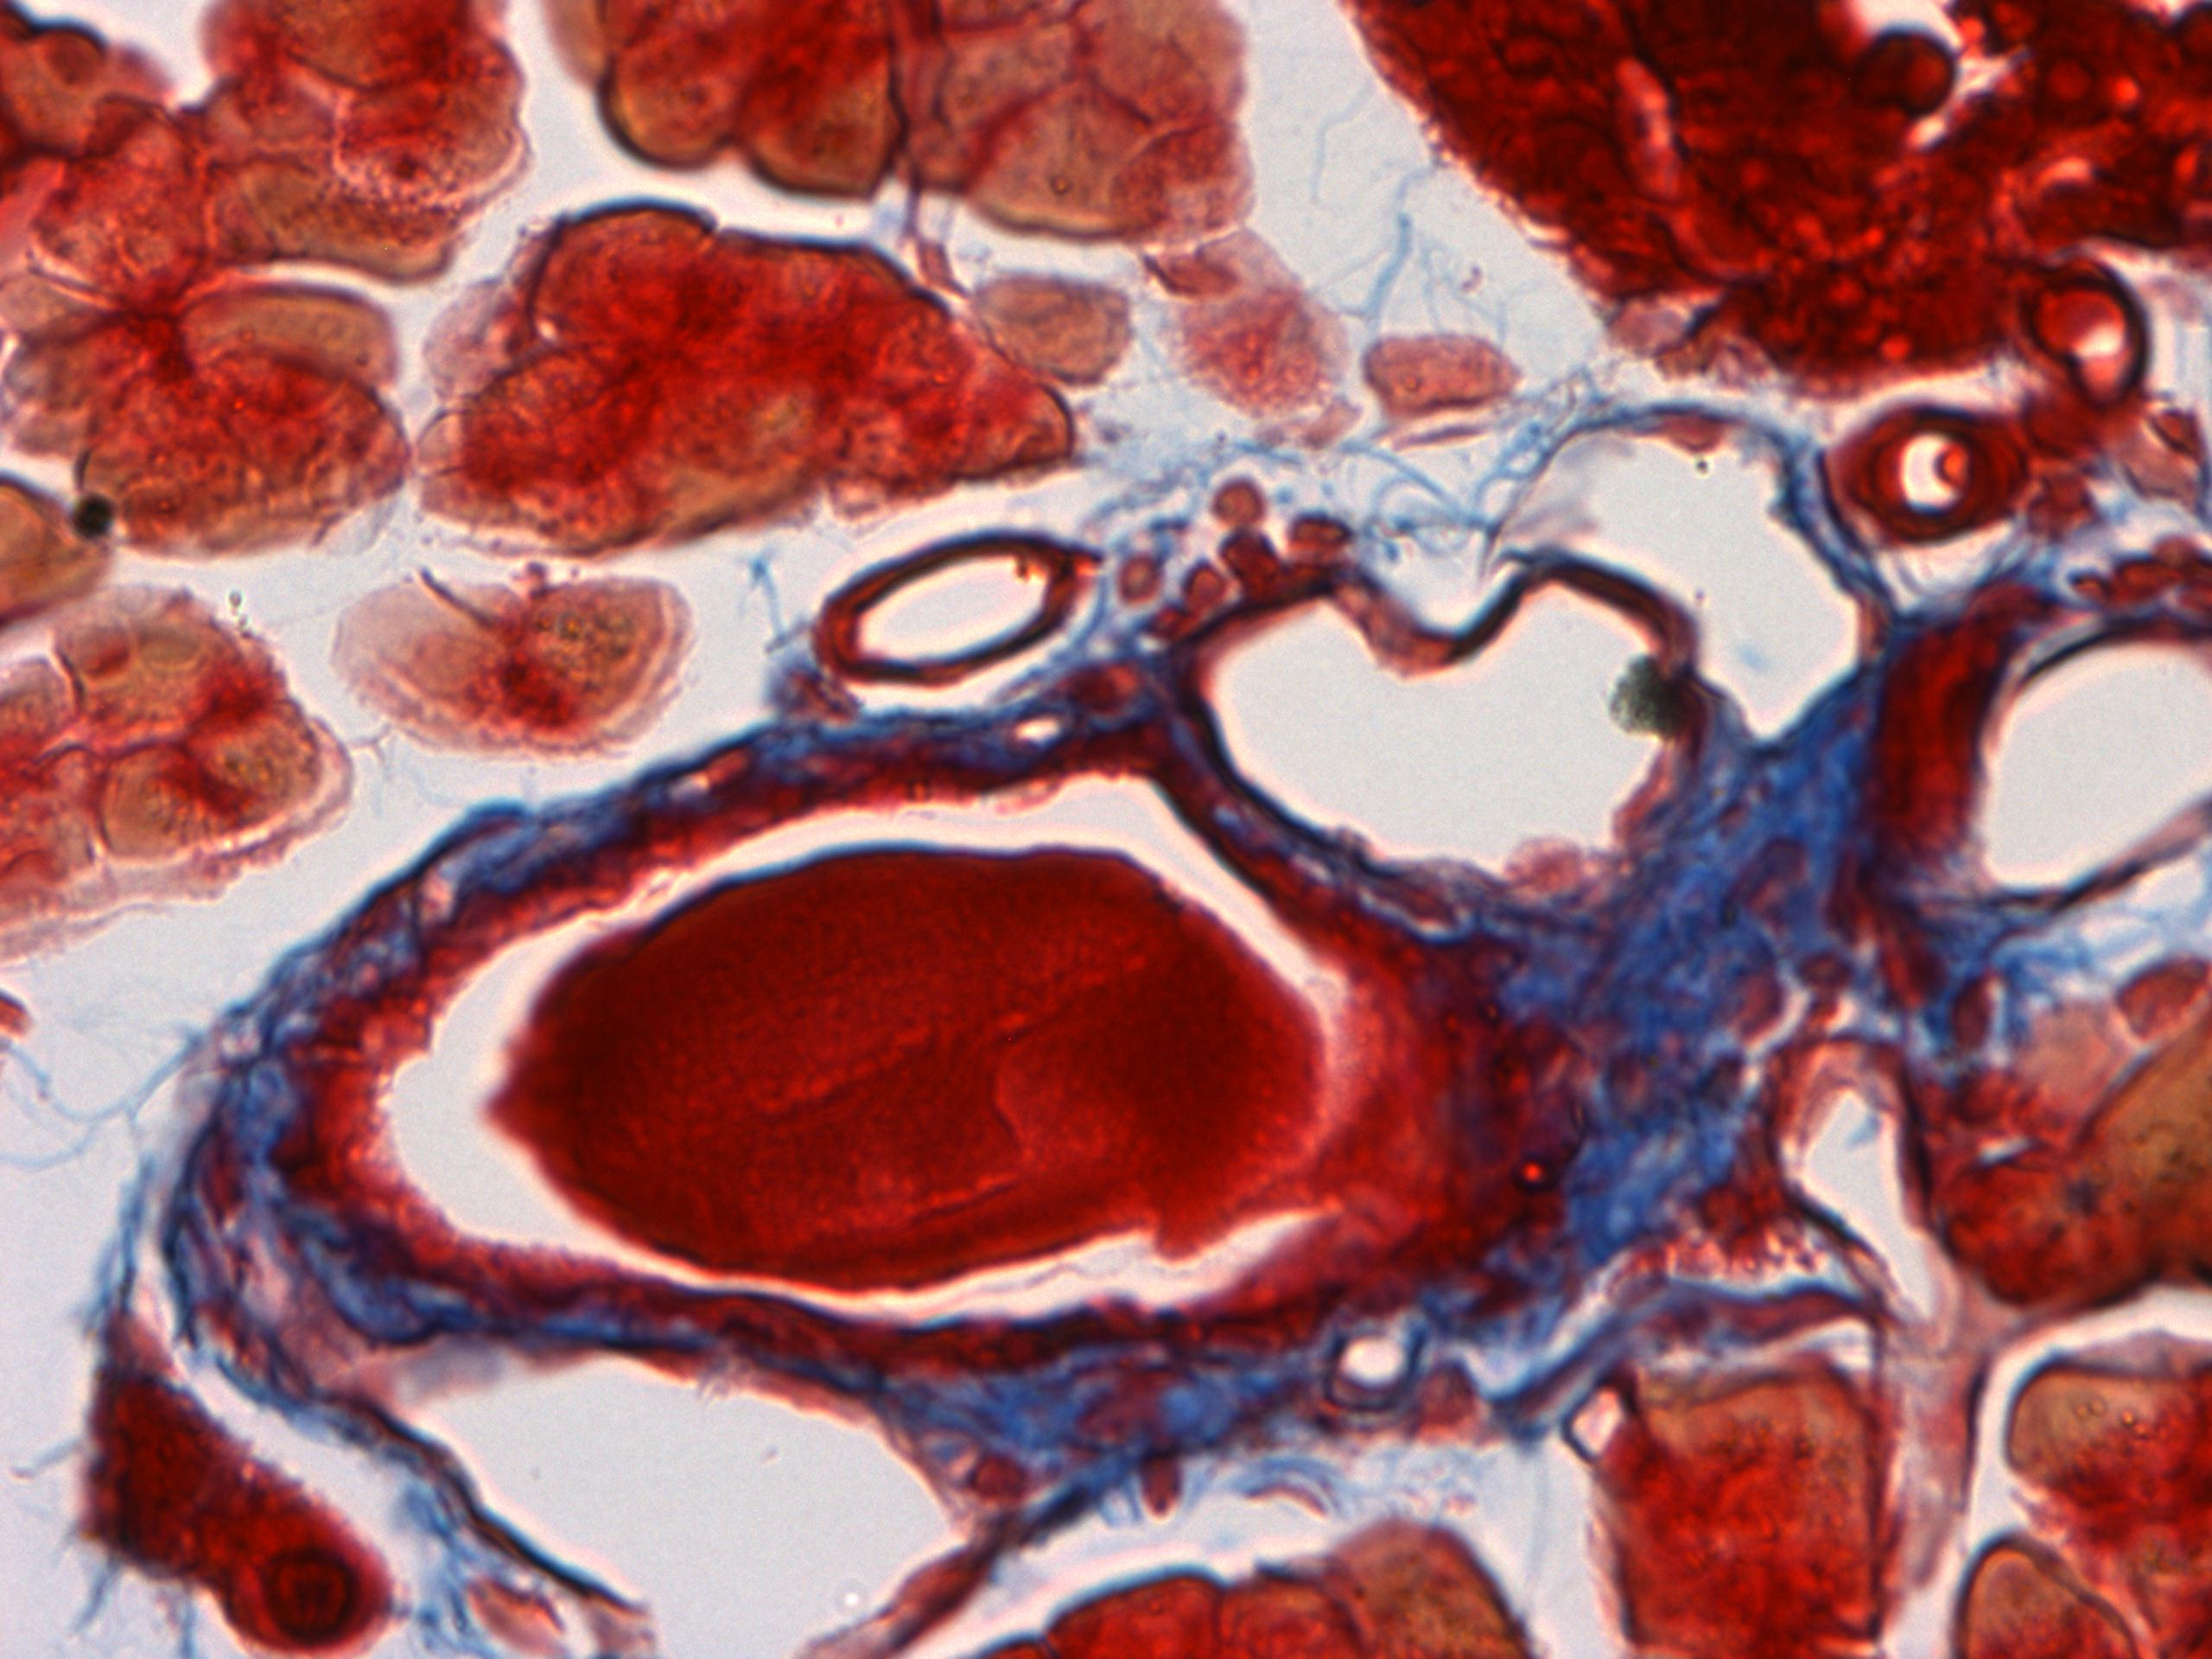
\includegraphics[width=86.2mm]{image/Tri-40x-2.jpg}
    \end{center}
    \psset{unit=4mm}
    \begin{pspicture}(-0.25,-0.75)(9.75,-0.75)
        \psaxes[ticks=x,tickstyle=top,Dx= 1,ticksize=1.5mm,labels=none](0,0)(10,0)
        \psaxes[ticks=x,tickstyle=top,Dx= 5,ticksize=2.5mm            ](0,0)(10,0)
        \psaxes[ticks=x,tickstyle=top,Dx=10,ticksize=3.5mm,labels=none](0,0)(10,0)
    \end{pspicture}
    \caption{Masson's trichrome 400x 之二}
    \label{blue-2}
\end{figure}

\begin{figure}
    \begin{center}
        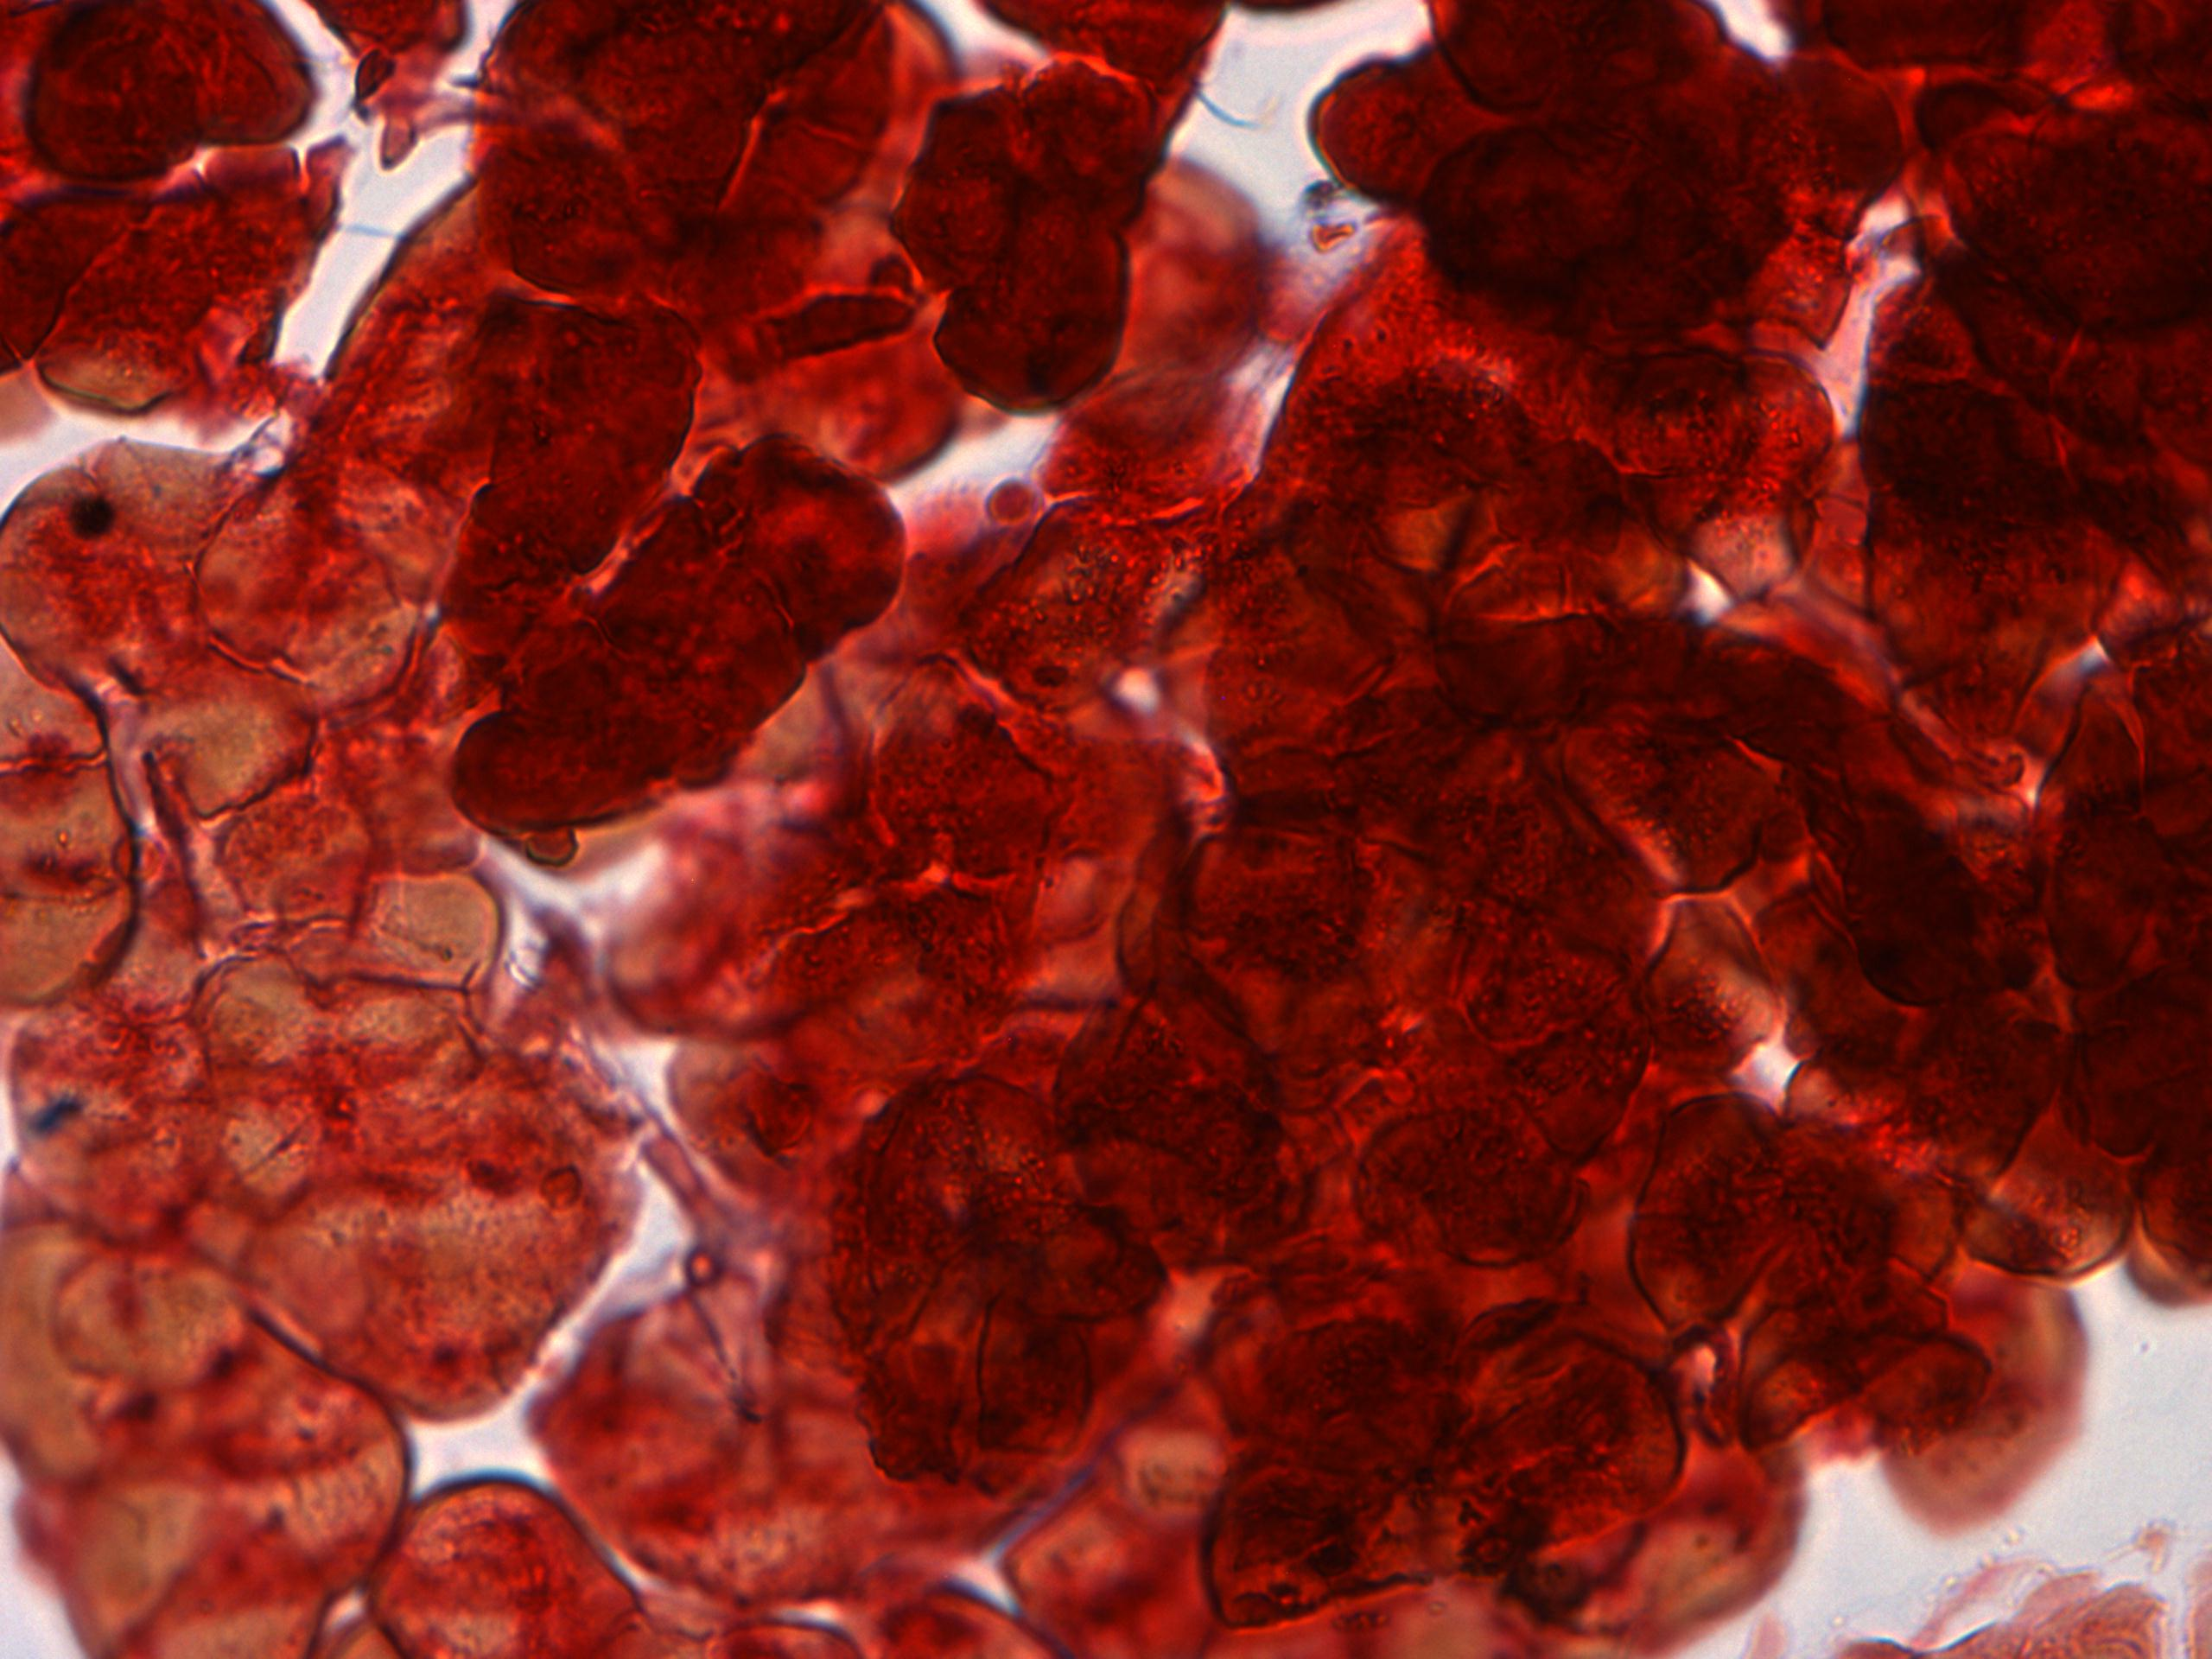
\includegraphics[width=86.2mm]{image/Tri-40x-3.jpg}
    \end{center}
    \psset{unit=4mm}
    \begin{pspicture}(-0.25,-0.75)(9.75,-0.75)
        \psaxes[ticks=x,tickstyle=top,Dx= 1,ticksize=1.5mm,labels=none](0,0)(10,0)
        \psaxes[ticks=x,tickstyle=top,Dx= 5,ticksize=2.5mm            ](0,0)(10,0)
        \psaxes[ticks=x,tickstyle=top,Dx=10,ticksize=3.5mm,labels=none](0,0)(10,0)
    \end{pspicture}
    \caption{Masson's trichrome 400x 之三}
\end{figure}

\section{討論}
\subsection{為什麼判讀為骨骼肌}
因為它看起來像好吃的牛排。

本片為縱切。肌纖維有一致的直徑,染成均勻的紅色,並可看出 epimysium, perimysium
與 endomysium 三層構造。較深染的細胞核靠近表面,且沒有肌間盤。

\subsection{片中的其他結構}
除了骨骼肌外,另有二種組織。一種是在 H\&E 與 Masson's trichrome 均染為紅色,內
有許多間隙的組織,見圖 \ref{red-1}, \ref{red-2} 及 \ref{red-3};另一種管狀組織
被 H\&E 染成紅色,但被 Massons's trichrome 染成藍色,見圖 \ref{blue-1} 及
\ref{blue-2}。

前者我想不出來是什麼東西,但後者應該是小靜脈。血管這種結締組織容易被 Masson's
trichrome 染藍,形狀又不圓,應該是小靜脈。

\end{document}
